
\documentclass[twoside]{article} % For LaTeX2e
\usepackage{aistats2022}

\usepackage[round]{natbib}
%\renewcommand{\bibname}{References}
%\renewcommand{\bibsection}{\subsubsection*{\bibname}}

% If you use BibTeX in apalike style, activate the following line:
\bibliographystyle{apalike}

% Optional math commands from https://github.com/goodfeli/dlbook_notation.
%%%%%% NEW MATH DEFINITIONS %%%%%

\usepackage{amsmath,amsfonts,bm}

% Mark sections of captions for referring to divisions of figures
\newcommand{\figleft}{{\em (Left)}}
\newcommand{\figcenter}{{\em (Center)}}
\newcommand{\figright}{{\em (Right)}}
\newcommand{\figtop}{{\em (Top)}}
\newcommand{\figbottom}{{\em (Bottom)}}
\newcommand{\captiona}{{\em (a)}}
\newcommand{\captionb}{{\em (b)}}
\newcommand{\captionc}{{\em (c)}}
\newcommand{\captiond}{{\em (d)}}

% Highlight a newly defined term
\newcommand{\newterm}[1]{{\bf #1}}


% Figure reference, lower-case.
\def\figref#1{figure~\ref{#1}}
% Figure reference, capital. For start of sentence
\def\Figref#1{Figure~\ref{#1}}
\def\twofigref#1#2{figures \ref{#1} and \ref{#2}}
\def\quadfigref#1#2#3#4{figures \ref{#1}, \ref{#2}, \ref{#3} and \ref{#4}}
% Section reference, lower-case.
\def\secref#1{section~\ref{#1}}
% Section reference, capital.
\def\Secref#1{Section~\ref{#1}}
% Reference to two sections.
\def\twosecrefs#1#2{sections \ref{#1} and \ref{#2}}
% Reference to three sections.
\def\secrefs#1#2#3{sections \ref{#1}, \ref{#2} and \ref{#3}}
% Reference to an equation, lower-case.
\def\eqref#1{equation~\ref{#1}}
% Reference to an equation, upper case
\def\Eqref#1{Equation~\ref{#1}}
% A raw reference to an equation---avoid using if possible
\def\plaineqref#1{\ref{#1}}
% Reference to a chapter, lower-case.
\def\chapref#1{chapter~\ref{#1}}
% Reference to an equation, upper case.
\def\Chapref#1{Chapter~\ref{#1}}
% Reference to a range of chapters
\def\rangechapref#1#2{chapters\ref{#1}--\ref{#2}}
% Reference to an algorithm, lower-case.
\def\algref#1{algorithm~\ref{#1}}
% Reference to an algorithm, upper case.
\def\Algref#1{Algorithm~\ref{#1}}
\def\twoalgref#1#2{algorithms \ref{#1} and \ref{#2}}
\def\Twoalgref#1#2{Algorithms \ref{#1} and \ref{#2}}
% Reference to a part, lower case
\def\partref#1{part~\ref{#1}}
% Reference to a part, upper case
\def\Partref#1{Part~\ref{#1}}
\def\twopartref#1#2{parts \ref{#1} and \ref{#2}}

\def\ceil#1{\lceil #1 \rceil}
\def\floor#1{\lfloor #1 \rfloor}
\def\1{\bm{1}}
\newcommand{\train}{\mathcal{D}}
\newcommand{\valid}{\mathcal{D_{\mathrm{valid}}}}
\newcommand{\test}{\mathcal{D_{\mathrm{test}}}}

\def\eps{{\epsilon}}


% Random variables
\def\reta{{\textnormal{$\eta$}}}
\def\ra{{\textnormal{a}}}
\def\rb{{\textnormal{b}}}
\def\rc{{\textnormal{c}}}
\def\rd{{\textnormal{d}}}
\def\re{{\textnormal{e}}}
\def\rf{{\textnormal{f}}}
\def\rg{{\textnormal{g}}}
\def\rh{{\textnormal{h}}}
\def\ri{{\textnormal{i}}}
\def\rj{{\textnormal{j}}}
\def\rk{{\textnormal{k}}}
\def\rl{{\textnormal{l}}}
% rm is already a command, just don't name any random variables m
\def\rn{{\textnormal{n}}}
\def\ro{{\textnormal{o}}}
\def\rp{{\textnormal{p}}}
\def\rq{{\textnormal{q}}}
\def\rr{{\textnormal{r}}}
\def\rs{{\textnormal{s}}}
\def\rt{{\textnormal{t}}}
\def\ru{{\textnormal{u}}}
\def\rv{{\textnormal{v}}}
\def\rw{{\textnormal{w}}}
\def\rx{{\textnormal{x}}}
\def\ry{{\textnormal{y}}}
\def\rz{{\textnormal{z}}}

% Random vectors
\def\rvepsilon{{\mathbf{\epsilon}}}
\def\rvtheta{{\mathbf{\theta}}}
\def\rva{{\mathbf{a}}}
\def\rvb{{\mathbf{b}}}
\def\rvc{{\mathbf{c}}}
\def\rvd{{\mathbf{d}}}
\def\rve{{\mathbf{e}}}
\def\rvf{{\mathbf{f}}}
\def\rvg{{\mathbf{g}}}
\def\rvh{{\mathbf{h}}}
\def\rvu{{\mathbf{i}}}
\def\rvj{{\mathbf{j}}}
\def\rvk{{\mathbf{k}}}
\def\rvl{{\mathbf{l}}}
\def\rvm{{\mathbf{m}}}
\def\rvn{{\mathbf{n}}}
\def\rvo{{\mathbf{o}}}
\def\rvp{{\mathbf{p}}}
\def\rvq{{\mathbf{q}}}
\def\rvr{{\mathbf{r}}}
\def\rvs{{\mathbf{s}}}
\def\rvt{{\mathbf{t}}}
\def\rvu{{\mathbf{u}}}
\def\rvv{{\mathbf{v}}}
\def\rvw{{\mathbf{w}}}
\def\rvx{{\mathbf{x}}}
\def\rvy{{\mathbf{y}}}
\def\rvz{{\mathbf{z}}}

% Elements of random vectors
\def\erva{{\textnormal{a}}}
\def\ervb{{\textnormal{b}}}
\def\ervc{{\textnormal{c}}}
\def\ervd{{\textnormal{d}}}
\def\erve{{\textnormal{e}}}
\def\ervf{{\textnormal{f}}}
\def\ervg{{\textnormal{g}}}
\def\ervh{{\textnormal{h}}}
\def\ervi{{\textnormal{i}}}
\def\ervj{{\textnormal{j}}}
\def\ervk{{\textnormal{k}}}
\def\ervl{{\textnormal{l}}}
\def\ervm{{\textnormal{m}}}
\def\ervn{{\textnormal{n}}}
\def\ervo{{\textnormal{o}}}
\def\ervp{{\textnormal{p}}}
\def\ervq{{\textnormal{q}}}
\def\ervr{{\textnormal{r}}}
\def\ervs{{\textnormal{s}}}
\def\ervt{{\textnormal{t}}}
\def\ervu{{\textnormal{u}}}
\def\ervv{{\textnormal{v}}}
\def\ervw{{\textnormal{w}}}
\def\ervx{{\textnormal{x}}}
\def\ervy{{\textnormal{y}}}
\def\ervz{{\textnormal{z}}}

% Random matrices
\def\rmA{{\mathbf{A}}}
\def\rmB{{\mathbf{B}}}
\def\rmC{{\mathbf{C}}}
\def\rmD{{\mathbf{D}}}
\def\rmE{{\mathbf{E}}}
\def\rmF{{\mathbf{F}}}
\def\rmG{{\mathbf{G}}}
\def\rmH{{\mathbf{H}}}
\def\rmI{{\mathbf{I}}}
\def\rmJ{{\mathbf{J}}}
\def\rmK{{\mathbf{K}}}
\def\rmL{{\mathbf{L}}}
\def\rmM{{\mathbf{M}}}
\def\rmN{{\mathbf{N}}}
\def\rmO{{\mathbf{O}}}
\def\rmP{{\mathbf{P}}}
\def\rmQ{{\mathbf{Q}}}
\def\rmR{{\mathbf{R}}}
\def\rmS{{\mathbf{S}}}
\def\rmT{{\mathbf{T}}}
\def\rmU{{\mathbf{U}}}
\def\rmV{{\mathbf{V}}}
\def\rmW{{\mathbf{W}}}
\def\rmX{{\mathbf{X}}}
\def\rmY{{\mathbf{Y}}}
\def\rmZ{{\mathbf{Z}}}

% Elements of random matrices
\def\ermA{{\textnormal{A}}}
\def\ermB{{\textnormal{B}}}
\def\ermC{{\textnormal{C}}}
\def\ermD{{\textnormal{D}}}
\def\ermE{{\textnormal{E}}}
\def\ermF{{\textnormal{F}}}
\def\ermG{{\textnormal{G}}}
\def\ermH{{\textnormal{H}}}
\def\ermI{{\textnormal{I}}}
\def\ermJ{{\textnormal{J}}}
\def\ermK{{\textnormal{K}}}
\def\ermL{{\textnormal{L}}}
\def\ermM{{\textnormal{M}}}
\def\ermN{{\textnormal{N}}}
\def\ermO{{\textnormal{O}}}
\def\ermP{{\textnormal{P}}}
\def\ermQ{{\textnormal{Q}}}
\def\ermR{{\textnormal{R}}}
\def\ermS{{\textnormal{S}}}
\def\ermT{{\textnormal{T}}}
\def\ermU{{\textnormal{U}}}
\def\ermV{{\textnormal{V}}}
\def\ermW{{\textnormal{W}}}
\def\ermX{{\textnormal{X}}}
\def\ermY{{\textnormal{Y}}}
\def\ermZ{{\textnormal{Z}}}

% Vectors
\def\vzero{{\bm{0}}}
\def\vone{{\bm{1}}}
\def\vmu{{\bm{\mu}}}
\def\vtheta{{\bm{\theta}}}
\def\va{{\bm{a}}}
\def\vb{{\bm{b}}}
\def\vc{{\bm{c}}}
\def\vd{{\bm{d}}}
\def\ve{{\bm{e}}}
\def\vf{{\bm{f}}}
\def\vg{{\bm{g}}}
\def\vh{{\bm{h}}}
\def\vi{{\bm{i}}}
\def\vj{{\bm{j}}}
\def\vk{{\bm{k}}}
\def\vl{{\bm{l}}}
\def\vm{{\bm{m}}}
\def\vn{{\bm{n}}}
\def\vo{{\bm{o}}}
\def\vp{{\bm{p}}}
\def\vq{{\bm{q}}}
\def\vr{{\bm{r}}}
\def\vs{{\bm{s}}}
\def\vt{{\bm{t}}}
\def\vu{{\bm{u}}}
\def\vv{{\bm{v}}}
\def\vw{{\bm{w}}}
\def\vx{{\bm{x}}}
\def\vy{{\bm{y}}}
\def\vz{{\bm{z}}}

% Elements of vectors
\def\evalpha{{\alpha}}
\def\evbeta{{\beta}}
\def\evepsilon{{\epsilon}}
\def\evlambda{{\lambda}}
\def\evomega{{\omega}}
\def\evmu{{\mu}}
\def\evpsi{{\psi}}
\def\evsigma{{\sigma}}
\def\evtheta{{\theta}}
\def\eva{{a}}
\def\evb{{b}}
\def\evc{{c}}
\def\evd{{d}}
\def\eve{{e}}
\def\evf{{f}}
\def\evg{{g}}
\def\evh{{h}}
\def\evi{{i}}
\def\evj{{j}}
\def\evk{{k}}
\def\evl{{l}}
\def\evm{{m}}
\def\evn{{n}}
\def\evo{{o}}
\def\evp{{p}}
\def\evq{{q}}
\def\evr{{r}}
\def\evs{{s}}
\def\evt{{t}}
\def\evu{{u}}
\def\evv{{v}}
\def\evw{{w}}
\def\evx{{x}}
\def\evy{{y}}
\def\evz{{z}}

% Matrix
\def\mA{{\bm{A}}}
\def\mB{{\bm{B}}}
\def\mC{{\bm{C}}}
\def\mD{{\bm{D}}}
\def\mE{{\bm{E}}}
\def\mF{{\bm{F}}}
\def\mG{{\bm{G}}}
\def\mH{{\bm{H}}}
\def\mI{{\bm{I}}}
\def\mJ{{\bm{J}}}
\def\mK{{\bm{K}}}
\def\mL{{\bm{L}}}
\def\mM{{\bm{M}}}
\def\mN{{\bm{N}}}
\def\mO{{\bm{O}}}
\def\mP{{\bm{P}}}
\def\mQ{{\bm{Q}}}
\def\mR{{\bm{R}}}
\def\mS{{\bm{S}}}
\def\mT{{\bm{T}}}
\def\mU{{\bm{U}}}
\def\mV{{\bm{V}}}
\def\mW{{\bm{W}}}
\def\mX{{\bm{X}}}
\def\mY{{\bm{Y}}}
\def\mZ{{\bm{Z}}}
\def\mBeta{{\bm{\beta}}}
\def\mPhi{{\bm{\Phi}}}
\def\mLambda{{\bm{\Lambda}}}
\def\mSigma{{\bm{\Sigma}}}

% Tensor
\DeclareMathAlphabet{\mathsfit}{\encodingdefault}{\sfdefault}{m}{sl}
\SetMathAlphabet{\mathsfit}{bold}{\encodingdefault}{\sfdefault}{bx}{n}
\newcommand{\tens}[1]{\bm{\mathsfit{#1}}}
\def\tA{{\tens{A}}}
\def\tB{{\tens{B}}}
\def\tC{{\tens{C}}}
\def\tD{{\tens{D}}}
\def\tE{{\tens{E}}}
\def\tF{{\tens{F}}}
\def\tG{{\tens{G}}}
\def\tH{{\tens{H}}}
\def\tI{{\tens{I}}}
\def\tJ{{\tens{J}}}
\def\tK{{\tens{K}}}
\def\tL{{\tens{L}}}
\def\tM{{\tens{M}}}
\def\tN{{\tens{N}}}
\def\tO{{\tens{O}}}
\def\tP{{\tens{P}}}
\def\tQ{{\tens{Q}}}
\def\tR{{\tens{R}}}
\def\tS{{\tens{S}}}
\def\tT{{\tens{T}}}
\def\tU{{\tens{U}}}
\def\tV{{\tens{V}}}
\def\tW{{\tens{W}}}
\def\tX{{\tens{X}}}
\def\tY{{\tens{Y}}}
\def\tZ{{\tens{Z}}}


% Graph
\def\gA{{\mathcal{A}}}
\def\gB{{\mathcal{B}}}
\def\gC{{\mathcal{C}}}
\def\gD{{\mathcal{D}}}
\def\gE{{\mathcal{E}}}
\def\gF{{\mathcal{F}}}
\def\gG{{\mathcal{G}}}
\def\gH{{\mathcal{H}}}
\def\gI{{\mathcal{I}}}
\def\gJ{{\mathcal{J}}}
\def\gK{{\mathcal{K}}}
\def\gL{{\mathcal{L}}}
\def\gM{{\mathcal{M}}}
\def\gN{{\mathcal{N}}}
\def\gO{{\mathcal{O}}}
\def\gP{{\mathcal{P}}}
\def\gQ{{\mathcal{Q}}}
\def\gR{{\mathcal{R}}}
\def\gS{{\mathcal{S}}}
\def\gT{{\mathcal{T}}}
\def\gU{{\mathcal{U}}}
\def\gV{{\mathcal{V}}}
\def\gW{{\mathcal{W}}}
\def\gX{{\mathcal{X}}}
\def\gY{{\mathcal{Y}}}
\def\gZ{{\mathcal{Z}}}

% Sets
\def\sA{{\mathbb{A}}}
\def\sB{{\mathbb{B}}}
\def\sC{{\mathbb{C}}}
\def\sD{{\mathbb{D}}}
% Don't use a set called E, because this would be the same as our symbol
% for expectation.
\def\sF{{\mathbb{F}}}
\def\sG{{\mathbb{G}}}
\def\sH{{\mathbb{H}}}
\def\sI{{\mathbb{I}}}
\def\sJ{{\mathbb{J}}}
\def\sK{{\mathbb{K}}}
\def\sL{{\mathbb{L}}}
\def\sM{{\mathbb{M}}}
\def\sN{{\mathbb{N}}}
\def\sO{{\mathbb{O}}}
\def\sP{{\mathbb{P}}}
\def\sQ{{\mathbb{Q}}}
\def\sR{{\mathbb{R}}}
\def\sS{{\mathbb{S}}}
\def\sT{{\mathbb{T}}}
\def\sU{{\mathbb{U}}}
\def\sV{{\mathbb{V}}}
\def\sW{{\mathbb{W}}}
\def\sX{{\mathbb{X}}}
\def\sY{{\mathbb{Y}}}
\def\sZ{{\mathbb{Z}}}

% Entries of a matrix
\def\emLambda{{\Lambda}}
\def\emA{{A}}
\def\emB{{B}}
\def\emC{{C}}
\def\emD{{D}}
\def\emE{{E}}
\def\emF{{F}}
\def\emG{{G}}
\def\emH{{H}}
\def\emI{{I}}
\def\emJ{{J}}
\def\emK{{K}}
\def\emL{{L}}
\def\emM{{M}}
\def\emN{{N}}
\def\emO{{O}}
\def\emP{{P}}
\def\emQ{{Q}}
\def\emR{{R}}
\def\emS{{S}}
\def\emT{{T}}
\def\emU{{U}}
\def\emV{{V}}
\def\emW{{W}}
\def\emX{{X}}
\def\emY{{Y}}
\def\emZ{{Z}}
\def\emSigma{{\Sigma}}

% entries of a tensor
% Same font as tensor, without \bm wrapper
\newcommand{\etens}[1]{\mathsfit{#1}}
\def\etLambda{{\etens{\Lambda}}}
\def\etA{{\etens{A}}}
\def\etB{{\etens{B}}}
\def\etC{{\etens{C}}}
\def\etD{{\etens{D}}}
\def\etE{{\etens{E}}}
\def\etF{{\etens{F}}}
\def\etG{{\etens{G}}}
\def\etH{{\etens{H}}}
\def\etI{{\etens{I}}}
\def\etJ{{\etens{J}}}
\def\etK{{\etens{K}}}
\def\etL{{\etens{L}}}
\def\etM{{\etens{M}}}
\def\etN{{\etens{N}}}
\def\etO{{\etens{O}}}
\def\etP{{\etens{P}}}
\def\etQ{{\etens{Q}}}
\def\etR{{\etens{R}}}
\def\etS{{\etens{S}}}
\def\etT{{\etens{T}}}
\def\etU{{\etens{U}}}
\def\etV{{\etens{V}}}
\def\etW{{\etens{W}}}
\def\etX{{\etens{X}}}
\def\etY{{\etens{Y}}}
\def\etZ{{\etens{Z}}}

% The true underlying data generating distribution
\newcommand{\pdata}{p_{\rm{data}}}
% The empirical distribution defined by the training set
\newcommand{\ptrain}{\hat{p}_{\rm{data}}}
\newcommand{\Ptrain}{\hat{P}_{\rm{data}}}
% The model distribution
\newcommand{\pmodel}{p_{\rm{model}}}
\newcommand{\Pmodel}{P_{\rm{model}}}
\newcommand{\ptildemodel}{\tilde{p}_{\rm{model}}}
% Stochastic autoencoder distributions
\newcommand{\pencode}{p_{\rm{encoder}}}
\newcommand{\pdecode}{p_{\rm{decoder}}}
\newcommand{\precons}{p_{\rm{reconstruct}}}

\newcommand{\laplace}{\mathrm{Laplace}} % Laplace distribution

\newcommand{\E}{\mathbb{E}}
\newcommand{\Ls}{\mathcal{L}}
\newcommand{\R}{\mathbb{R}}
\newcommand{\emp}{\tilde{p}}
\newcommand{\lr}{\alpha}
\newcommand{\reg}{\lambda}
\newcommand{\rect}{\mathrm{rectifier}}
\newcommand{\softmax}{\mathrm{softmax}}
\newcommand{\sigmoid}{\sigma}
\newcommand{\softplus}{\zeta}
\newcommand{\KL}{D_{\mathrm{KL}}}
\newcommand{\Var}{\mathrm{Var}}
\newcommand{\standarderror}{\mathrm{SE}}
\newcommand{\Cov}{\mathrm{Cov}}
% Wolfram Mathworld says $L^2$ is for function spaces and $\ell^2$ is for vectors
% But then they seem to use $L^2$ for vectors throughout the site, and so does
% wikipedia.
\newcommand{\normlzero}{L^0}
\newcommand{\normlone}{L^1}
\newcommand{\normltwo}{L^2}
\newcommand{\normlp}{L^p}
\newcommand{\normmax}{L^\infty}

\newcommand{\parents}{Pa} % See usage in notation.tex. Chosen to match Daphne's book.

\DeclareMathOperator*{\argmax}{arg\,max}
\DeclareMathOperator*{\argmin}{arg\,min}

\DeclareMathOperator{\sign}{sign}
\DeclareMathOperator{\Tr}{Tr}
\let\ab\allowbreak


\usepackage{amsmath,amssymb,amsthm}
\usepackage{unicode-math}
\usepackage{mathtools}
\setmathfont{STIX2Math.otf}
\usepackage{dsfont}

\usepackage{proof-at-the-end}
\newtheorem{remark}{\textbf{Remark}}
\newtheorem{lemma}{\textbf{Lemma}}
\newtheorem{assumption}{\textbf{A}}
\newtheorem{theorem}{\textbf{Theorem}}
\newtheorem{proposition}{\textbf{Proposition}}
\newtheorem{definition}{\textbf{Definition}}

\pgfkeys{/prAtEnd/global custom defaults/.style={
    %proof at the end,
    end,
    %normal,
    restate,
    text link={\textit{Proof.} The proof is in the \textit{supplementary material}.
    }
  }
% Fix link later for camera ready version.
}

\def\code#1{\texttt{#1}}
\DeclareMathOperator*{\minimize}{minimize}
\DeclareMathOperator*{\maximize}{maximize}
\DeclareMathOperator*{\argmax}{arg\,max}
\DeclareMathOperator*{\argmin}{arg\,min} 

\newcommand*\xbar[1]{%
  \hbox{%
    \vbox{%
      \hrule height 0.6pt % The actual bar
      \kern0.33ex%         % Distance between bar and symbol
      \hbox{%
        \kern-0.1em%      % Shortening on the left side
        \ensuremath{#1}%
        \kern-0.1em%      % Shortening on the right side
      }%
    }%
  }%
} 

\newcommand{\E}[1]{\mathbb{E}\left[\,#1\,\right]}
\newcommand{\Esub}[2]{\mathbb{E}_{#1}\left[\,#2\,\right]}
\newcommand{\V}[1]{\mathbb{V}\left[\,#1\,\right]}
\newcommand{\Vsub}[2]{\mathbb{V}_{#1}\left[\,#2\,\right]}
\newcommand{\Cov}[1]{\mathrm{Cov}\left(\,#1\,\right)}
\newcommand{\Covsub}[2]{\mathrm{Cov}_{#1}\left(\,#2\,\right)}
\newcommand{\Corr}[1]{\mathrm{Corr}\left(\,#1\,\right)}

\newcommand{\Df}[2]{D_{f}(#1\parallel#2)}
\newcommand{\DKL}[2]{D_{\mathrm{KL}}(#1\parallel#2)}
\newcommand{\DChi}[2]{D_{\chi^2}(#1\paallel#2)}
\newcommand{\DTV}[2]{{\parallel#1 - #2\parallel}_{\mathrm{TV}}}

\newcommand{\vX}{\symbfup{X}}
\newcommand{\vY}{\symbfup{Y}}
\newcommand{\vZ}{\symbfup{Z}}

\newcommand{\va}{\symbfup{a}}
\newcommand{\vb}{\symbfup{b}}
\newcommand{\vc}{\symbfup{c}}
\newcommand{\vd}{\symbfup{d}}
\newcommand{\ve}{\symbfup{e}}
\newcommand{\vf}{\symbfup{f}}
\newcommand{\vg}{\symbfup{g}}
\newcommand{\vh}{\symbfup{h}}
\newcommand{\vi}{\symbfup{i}}
\newcommand{\vj}{\symbfup{j}}
\newcommand{\vk}{\symbfup{k}}
\newcommand{\vl}{\symbfup{l}}
\newcommand{\vm}{\symbfup{m}}
\newcommand{\vn}{\symbfup{n}}
\newcommand{\vo}{\symbfup{o}}
\newcommand{\vp}{\symbfup{p}}
\newcommand{\vq}{\symbfup{q}}
\newcommand{\vr}{\symbfup{r}}
\newcommand{\vs}{\symbfup{s}}
\newcommand{\vt}{\symbfup{t}}
\newcommand{\vu}{\symbfup{u}}
\newcommand{\vv}{\symbfup{v}}
\newcommand{\vw}{\symbfup{w}}
\newcommand{\vx}{\symbfup{x}}
\newcommand{\vy}{\symbfup{y}}
\newcommand{\vz}{\symbfup{z}}
\newcommand{\valpha}{\symbfup{\alpha}}
\newcommand{\vmu}{\symbfup{\mu}}
\newcommand{\vtheta}{\symbfup{\theta}}
\newcommand{\vlambda}{\symbfup{\lambda}}

\newcommand{\mA}{\symbfup{A}}
\newcommand{\mB}{\symbfup{B}}
\newcommand{\mC}{\symbfup{C}}
\newcommand{\mD}{\symbfup{D}}
\newcommand{\mE}{\symbfup{E}}
\newcommand{\mF}{\symbfup{F}}
\newcommand{\mG}{\symbfup{G}}
\newcommand{\mH}{\symbfup{H}}
\newcommand{\mI}{\symbfup{I}}
\newcommand{\mJ}{\symbfup{J}}
\newcommand{\mK}{\symbfup{K}}
\newcommand{\mL}{\symbfup{L}}
\newcommand{\mM}{\symbfup{M}}
\newcommand{\mN}{\symbfup{N}}
\newcommand{\mO}{\symbfup{O}}
\newcommand{\mP}{\symbfup{P}}
\newcommand{\mQ}{\symbfup{Q}}
\newcommand{\mR}{\symbfup{R}}
\newcommand{\mS}{\symbfup{S}}
\newcommand{\mT}{\symbfup{T}}
\newcommand{\mU}{\symbfup{U}}
\newcommand{\mV}{\symbfup{V}}
\newcommand{\mW}{\symbfup{W}}
\newcommand{\mX}{\symbfup{X}}
\newcommand{\mY}{\symbfup{Y}}
\newcommand{\mZ}{\symbfup{Z}}

\newcommand{\iprod}[2]{\langle #1, #2 \rangle}
\newcommand{\ind}[1]{\mathds{1}_{#1}}


\usepackage{xcolor}         % hyperlinks
\usepackage{amsfonts}       % blackboard math symbols
\usepackage{nicefrac}       % compact symbols for 1/2, etc.
\usepackage{microtype}      % microtypography
\usepackage{setspace}
\usepackage{wrapfig}
\usepackage[inline]{enumitem}
\usepackage{caption}     
\usepackage{subcaption}     
\usepackage{float}     
%\usepackage[15-]{pagesel}

\usepackage{minted}
%\usepackage{newunicodechar}
%\setmonofont{DejaVu Sans Mono}[Scale=MatchLowercase]

%% Tikz corner
\usepackage{tikz}
\usepackage{pgf}
\usepackage{pgfplots}
\usepackage{pgfplotstable}

\usetikzlibrary{patterns}
\usetikzlibrary{fit, calc}
\usepgfplotslibrary{fillbetween}
\usepgfplotslibrary{groupplots}
\usepgfplotslibrary{statistics}
\usepgfplotslibrary{external} 

\usepackage{pifont}
\usepackage{xcolor}
\newcommand{\cmark}{\textcolor{green!80!black}{\ding{51}}}
\newcommand{\xmark}{\textcolor{red}{\ding{55}}}

\tikzset{external/system call={lualatex -shell-escape -halt-on-error -interaction=batchmode -jobname "\image" "\texsource"}}

\begin{document}

% If your paper is accepted and the title of your paper is very long,
% the style will print as headings an error message. Use the following
% command to supply a shorter title of your paper so that it can be
% used as headings.
%
%\runningtitle{I use this title instead because the last one was very long}

% If your paper is accepted and the number of authors is large, the
% style will print as headings an error message. Use the following
% command to supply a shorter version of the authors names so that
% they can be used as headings (for example, use only the surnames)
%
%\runningauthor{Surname 1, Surname 2, Surname 3, ...., Surname n}

\twocolumn[
\aistatstitle{Markov-Chain Monte Carlo Score Estimators for \\ Variational Inference with Score Climbing}
\aistatsauthor{Kyurae Kim \And Jisu Oh \And Hongseok Kim }
\aistatsaddress{Sogang University} ]

\begin{abstract}
  
Markovian score climbing (MSC) is a recently proposed variational inference (VI) method based on Markov-chain Monte Carlo (MCMC) for minimizing the inclusive Kullback-Leibler (KL) divergence.
In this paper, we show that, when combined with independent Metropolis-Hastings (IMH) type of kernels, MSC has interesting properties.
Specifically, IMH kernels can automatically trade off bias and variance when used in MSC.
Also, we show that the variance of the conditional importance sampling kernel, which was originally proposed for MSC, can increase with an additional computational budget.
To fix this, we propose to use parallel IMH (PIMH) chains for obtaining stochastic gradients.
We find that MSC with PIMH achieves better performance faster compared to other inclusive and exclusive VI methods.
%Our results motivate the use of the inclusive KL divergence for VI.

%%% Local Variables:
%%% TeX-master: "master"
%%% End:

\end{abstract}


\section{Introduction}\label{section:intro}
Bayesian inference aims to analyze the posterior distribution of an unknown latent variable \(\vz\) from which the data \(\vx\) is observed.
%
%\jrg{I don't know that I'd call these latent variables in the most general setting. Historically, these were more commonly parameters of a model $\theta$. I also think $\vz$ here clashes with the use of $\vz$ later to mean the samples from the Markov chain}.
% krk: The papers closest to our work seems to prefer the term "latent variable" even though they still consider the general Bayesian inference setting. So I think it's okay to match the terminology with those. Also, I think \(\vz\) here is the same as the samples from the Markov chain, is this confusing here?
%
By assuming a model \(p\,(\vx\,|\,\vz)\), the posterior \(\pi\,(\vz)\) is given by Bayes' rule such that \(\pi\,(\vz) = {p\,(\vx\,|\,\vz)\,p\,(\vz)}/{p\,(\vx)}\) where \(p\,(\vz)\) represents our prior belief on \(\vz\).
Instead of working directly with the target distribution \(\pi\), variational inference (VI,~\citealt{blei_variational_2017}) seeks a \textit{variational approximation} \(q\,(\vz; \vlambda)\) that is the most similar to \(\pi\) according to a discrepancy measure \(D\,(\pi,\, q(\cdot; \vlambda))\).

Naturally, choosing an appropriate discrepancy measure is key to the quality of the solution.
This fact has led to a quest for suitable divergence measures~\citep{pmlr-v37-salimans15, NIPS2016_7750ca35, NIPS2017_35464c84, NEURIPS2018_1cd138d0, pmlr-v97-ruiz19a}.
So far, the exclusive (or reverse, backward)  KL divergence \(\DKL{q\left(\cdot; \vlambda\right)}{\pi}\) has been used ``exclusively'' among various discrepancy measures.
This is partly because the exclusive KL is defined as an average over \(q_{\lambda}(\vz)\), which can be approximated efficiently.
In contrast, the inclusive KL defined as
%
{%\small
\vspace{-0.05in}
\begin{align*}
  \DKL{\pi}{q\left(\cdot; \vlambda\right)}
  = \int \pi\,(\vz) \log \frac{\pi\left(\vz\right)}{\,q(\vz; \vlambda)} \,d\vz
  = \Esub{\rvvz \sim \pi\left(\cdot\right)}{\log \frac{\pi\left(\rvvz\right)}{\,q(\rvvz; \vlambda)} } %\label{eq:klpq}
\end{align*}
%\vspace{-0.05in}
}%
%
requires to take the integral over \(\pi\).
Since our goal is to obtain \(\pi\) in the first place, the difficulty of minimizing the inclusive KL lies in the fact that this is a chicken-and-egg problem.
Despite this challenge, the inclusive KL has consistently drawn attention due to its statistical properties~\citep{minka2005divergence, mackay_local_2001}.

Recently,~\citet{NEURIPS2020_b2070693,pmlr-v124-ou20a} have respectively proposed Markovian score climbing (MSC) and joint stochastic approximation (JSA).
These methods minimize the inclusive KL using stochastic gradient descent (SGD,~\citealt{robbins_stochastic_1951}) where the gradients are estimated using Markov chain Monte Carlo (MCMC).
The MCMC kernel \(K_{\vlambda_t}\left(\vz_t, \cdot\right)\) is chosen such that it directly takes advantage of the current variational approximation \(q\left(\cdot; \vlambda_t\right)\).
Thus, the quality of the gradients improves over time as the KL divergence decreases.
Still, the gradients are non-asymptotically biased and Markovian, which sharply contrasts MSC and JSA from classical black-box VI~\citep{pmlr-v33-ranganath14, JMLR:v18:16-107}, where the gradients are independent and unbiased.
While~\citet{NEURIPS2020_b2070693} has shown convergence of MSC through the work of~\citet{gu_stochastic_1998}, this result is only asymptotic and does not provide insight into the practical performance of MSC.

%

In this paper, we address these theoretical gaps by casting MSC and JSA into a general framework we call Markov chain score ascent (MCSA), which we show is a special case of Markov chain gradient descent (MCGD,~\citealt{duchi_ergodic_2012}).
This enables the application of the non-asymptotic convergence results of MCGD~\citep{duchi_ergodic_2012, NEURIPS2018_1371bcce, pmlr-v99-karimi19a, doan_finitetime_2020, doan_convergence_2020, Xiong_Xu_Liang_Zhang_2021, debavelaere_convergence_2021}.
For MCGD methods, the fundamental properties affecting the convergence rate are the ergodic convergence rate (\(\rho\)) of the MCMC kernel and the gradient variance (\(G\)).
We analyze \(\rho\) and \(G\) of MSC and JSA, enabling their practical comparison given a fixed computational budget (\(N\)).
Furthermore, based on the recent insight that the mixing rate does not affect the convergence rate of MCGD~\citet{doan_convergence_2020,doan_finitetime_2020}, we propose a novel scheme, parallel MCSA (pMCSA), which achieves lower variance by trading off the mixing rate.
We verify our theoretical analysis through numerical simulations and compare MSC, JSA, and pMCSA on general Bayesian inference problems.
Our experiments show that our proposed method is superior to previous MCSA approaches.
%Furthermore, MSCA is competitive against evidence lower-bound (ELBO) maximization within our experiments.
%We further discuss this result in relation with the conclusions of~\citet{dhaka_challenges_2021} in~\cref{section:discussion}.

\vspace{-0.1in}
\paragraph{Contribution Summary}
%\jrg{Item one should be something along the lines of we provide the first non-asymptotic analysis of MSC and JSA. Item two should be we accomplish this by showing it's a special case (basically point 1 below). I've sketched this out -- maybe we add back in the appropriate sec/thm references?}
%\vspace{-0.2in}
%% \begin{enumerate*}[label=\textbf{(\roman*)}]
\setlength\itemsep{0.01in}
\begin{enumerate}[leftmargin=7mm,listparindent=\parindent]
    \item We provide the first non-asymptotic theoretical analysis of two recently proposed inclusive KL minimization methods, MSC and JSA \textbf{(\cref{section:convergence,thm:product_kernel})}.
    \item To accomplish this, we show that both methods can be viewed as what we call ``Markov chain score ascent'' (MCSA) methods, which are a specical case of the MCGD framework \textbf{(\cref{section:comparison,thm:jsa,thm:msc})}.
    \item In light of this, we develop a novel MCSA method which we call parallel MCSA (pMCSA) that achieves lower gradient variance.
    \item We demonstrate that pMCSA achieves superior empirical performance across a variety of Bayesian inference tasks \textbf{(\cref{section:eval})}.
\end{enumerate}

%%% Local Variables:
%%% TeX-master: "master"
%%% End:


\section{Background}
\vspace{-0.05in}
\subsection{Inclusive Variational Inference Until Now}\label{section:ivi_previous}
\vspace{-0.05in}
A typical way to perform VI is to use stochastic gradient descent (SGD,~\citealt{robbins_stochastic_1951, bottou_online_1999}), which requires unbiased gradient estimates of the optimization target.
In the case of inclusive variational inference, this corresponds to estimating
%
\begin{align}
  \nabla_{\vlambda} \DKL{p}{q_{\lambda}}
  = \Esub{p(\vz\mid\vx)}{ - \nabla_{\vlambda} \log q_{\vlambda}(\vz) }
  = - \Esub{p(\vz\mid\vx)}{ s\,(\vz; \vlambda) }
\end{align}
where \(s\,(\vz; \vlambda) = \nabla_{\vlambda} \log q_{\vlambda}(\vz)\) is known as the \textit{score function}.
Evidently, estimating \(\nabla_{\vlambda} \DKL{p}{q_{\lambda}}\) requires integrating the score function over \(p(\vz\mid\vx)\), which is prohibitive.

\vspace{-0.1in}
\paragraph{Importance Sampling}
When the variational approximation \(q_{\lambda}\) is easy to sample from, one can use importance sampling (IS, \citealt{robert_monte_2004, mcbook}) since 
\begin{align}
  \Esub{p(\vz\mid\vx)}{ s\,(\vz; \vlambda) }
  \propto \Esub{q_{\vlambda}}{ w\,(\vz) \, s\,(\vz; \vlambda) }
  \approx \frac{1}{N} \sum^{N}_{i=1} w\,(\vz^{(i)}) \, s\,(\vz^{(i)}; \vlambda) .
\end{align}
where \(w\,(\vz) = p\,(\vz,\vx) / q_{\vlambda}(\vz)\) is known as the \textit{importance weight}, and \(\vz^{(1)},\, \ldots,\, \vz^{(N)}\) are \(N\) independent samples from \(q_{\vlambda}(\vz)\).
This scheme is equivalent to adaptive IS methods~\citep{cappe_adaptive_2008, bugallo_adaptive_2017} since the IS proposal \(q_{\vlambda}(\vz)\) is iteratively optimized based on the current samples.
Though IS is unbiased, it is highly unstable in practice.
A more stable alternative is to use the \textit{normalized weight} \(\widetilde{w}^{(i)} = \nicefrac{w\,(\vz^{(i)})}{\sum_{i=1}^N w\,(\vz^{(i)}) }\), resulting in the self-normalized IS (SNIS) approximation.
Unfortunately, SNIS still fails to converge even on moderate dimensional objectives, and unlike IS, is no longer unbiased~\citep{robert_monte_2004, mcbook}.

\vspace{-0.1in}
%
  \begin{minipage}[l]{0.45\linewidth}
    \small
    \centering
    \begin{algorithm2e}[H]
      \DontPrintSemicolon
      \SetAlgoLined
      \KwIn{MCMC kernel \(K(\vz,\cdot)\),
        initial sample \(\vz_0\),
        initial parameter \(\vlambda_0\),
        number of iterations \(T\),
        stepsize schedule \(\gamma_t\)}
      \For{\textcolor{black}{\(t = 1, 2, \ldots, T\)}}{
        \textit{Sample} \hspace{0.035in} \( \vz_{t} \sim K(\vz_{t-1}, \cdot) \)\;
        \textit{Estimate} \( s(\vz; \vlambda) = \nabla_{\vlambda} \log q_{\vlambda}(\vz_t) \)\;
        \textit{Update} \hspace{0.03in} \( \vlambda_{t} = \vlambda_{t-1} + \gamma_t\, s\,(\vz_t;\vlambda_{t-1}) \)\;
      }
      \caption{Markovian Score Climbing}\label{alg:msc}
    \end{algorithm2e}
    \vspace{-0.1in}
  \end{minipage}
  \qquad
  \begin{minipage}[r]{0.5\linewidth}
    \vspace{-0.1in}
    \begin{figure}[H]
      \centering
      
\begin{tikzpicture}
  \begin{axis}[
      legend style={
        draw=none,
        fill=none,
        at=({current bounding box.north-|.5,0}),
        anchor=south,
      },
      legend cell align={left},
      %xmode=log,
      xlabel={Iteration},
      %ylabel={Trace},
      tick pos=left,
      tick align={outside},
      major tick length={2pt},
      axis line style={thick},
      every tick/.style={black, thick},
      xmin=1,
      xmax=500,
      ymin=-1.5,
      ymax=8.5,
      xtick={1, 100, 200, 300, 400, 500},
      %xticklabels={\(2^{5}\), \(2^{6}\), \(2^{7}\), \(2^{8}\), \(2^{9}\), \(2^{12}\)},
      %x dir=reverse,
      %table/col sep=comma,
      height={4cm},
      width={6.0cm},
    ]

    %% Thick lines
    \addplot [thick, red, mark size=2pt] coordinates {
(1,3.7744966552635417)
(2,6.6637992482529524)
(3,6.259990698592114)
(4,5.997717299544704)
(5,5.798112583190721)
(6,5.536690619969111)
(7,5.384524538240413)
(8,5.275574413902902)
(9,6.243033825159706)
(10,6.045791493861715)
(11,5.905188012235524)
(12,5.7947743141303745)
(13,5.703422931858933)
(14,8.469885134555476)
(15,8.227143565336176)
(16,7.342984877784093)
(17,7.243116624848073)
(18,7.155390820622436)
(19,7.178898516479454)
(20,7.089021416378296)
(21,7.008796826321647)
(22,7.997167461547135)
(23,7.898886397906378)
(24,7.809385491279324)
(25,7.727274144084045)
(26,7.651459545353988)
(27,7.581067456656407)
(28,7.515387789323801)
(29,7.453836168874047)
(30,7.395926142060064)
(31,7.341248664581308)
(32,7.289456688876174)
(33,7.240253399475244)
(34,7.1933831054477055)
(35,7.148624100384867)
(36,7.10578300088166)
(37,7.064690210863979)
(38,7.025196253605488)
(39,6.987168779851843)
(40,6.950490108091594)
(41,6.915055187553156)
(42,6.88076989988074)
(43,6.847549634301591)
(44,6.815318085267477)
(45,6.7840062323083865)
(46,6.753551470075622)
(47,6.723896862918796)
(48,6.617974367341658)
(49,6.588663118009894)
(50,6.560133738483243)
(51,6.53232580294924)
(52,6.505185180776635)
(53,7.086144053463915)
(54,7.053330601491464)
(55,7.021590266940274)
(56,6.9908242549989055)
(57,6.96094663638384)
(58,6.9318820776879)
(59,6.9035640850973525)
(60,6.8759336203764345)
(61,7.014231450491013)
(62,6.986201373565165)
(63,6.958801249509174)
(64,6.931993237170517)
(65,6.9057425215538855)
(66,6.880017012245051)
(67,6.85478707800088)
(68,6.830025312434275)
(69,6.805706326532405)
(70,6.781806564411765)
(71,6.758304139262528)
(72,6.735178686889957)
(73,6.712411234639783)
(74,6.689984083811594)
(75,6.667880703930543)
(76,6.64608563747212)
(77,6.624584413824602)
(78,6.603363471434953)
(79,6.5824100872211995)
(80,6.561712312451603)
(81,6.5412589143914746)
(82,6.521039323104858)
(83,6.50104358287279)
(84,6.481262307754261)
(85,6.461686640871737)
(86,6.442308217051617)
(87,6.423119128492223)
(88,6.404111893168742)
(89,6.385279425716841)
(90,6.3666150105649075)
(91,6.348112277109757)
(92,6.329765176752502)
(93,6.311567961630603)
(94,6.293515164899163)
(95,6.2756015824296405)
(96,6.257822255807558)
(97,6.2401724565226555)
(98,6.22264767125555)
(99,6.205243588174375)
(100,6.187956084163267)
(101,6.170781212912098)
(102,6.153671126843844)
(103,6.136419931382466)
(104,6.119036785809355)
(105,6.064959739335891)
(106,6.046831896859059)
(107,6.028687447161313)
(108,6.010535278933221)
(109,5.992379731321853)
(110,5.974134891383233)
(111,5.955812895881109)
(112,5.937420230175251)
(113,5.9189604925332375)
(114,5.900435500996035)
(115,5.881814695282706)
(116,5.8631132600438844)
(117,5.8443975022639565)
(118,5.825669716106254)
(119,5.806931346411407)
(120,5.788137282007762)
(121,5.769290013827989)
(122,5.750391217071285)
(123,5.7313312876144265)
(124,5.712119241561277)
(125,5.692763481548353)
(126,5.6732718189835065)
(127,5.653651480729689)
(128,5.633909110123747)
(129,5.614050768747075)
(130,5.594081942797848)
(131,5.574007556005396)
(132,5.553831989643474)
(133,5.533559109250085)
(134,5.513192297069295)
(135,5.492734488920092)
(136,5.472188214098125)
(137,5.451555636963526)
(138,5.430838599007848)
(139,5.410038660381831)
(140,5.389157140071637)
(141,5.368195154112285)
(142,5.347153651409994)
(143,5.326033446902893)
(144,5.304835251919728)
(145,5.283559701699293)
(146,5.262207380111723)
(147,5.2407788416798065)
(148,5.219274631037527)
(149,5.197672437295372)
(150,5.175970520592031)
(151,5.154167161853462)
(152,5.13226067332589)
(153,5.110249408626393)
(154,5.0881688398692315)
(155,5.06601732551165)
(156,5.043793266659102)
(157,5.021495112993182)
(158,4.999121368886506)
(159,4.976670599722386)
(160,4.954141438428249)
(161,5.191006290169998)
(162,5.14400742059719)
(163,5.101685252488614)
(164,5.062686948459874)
(165,5.026166818537952)
(166,4.991556348247825)
(167,4.958452797003244)
(168,4.926559254683935)
(169,4.8956498277572855)
(170,4.865548209565154)
(171,4.836113870945296)
(172,4.807232825507383)
(173,4.778811261861212)
(174,4.75077103748358)
(175,4.723046417753763)
(176,4.69558166879905)
(177,4.668329248206368)
(178,4.641248421876633)
(179,4.614304189242829)
(180,4.587466434543097)
(181,4.560709245717947)
(182,4.534010358917163)
(183,4.507350698101204)
(184,4.480713987408027)
(185,4.4540864198622225)
(186,4.427456370308532)
(187,4.523628310287821)
(188,4.486699536043139)
(189,4.450735375209012)
(190,4.415594926155893)
(191,4.3811593359719705)
(192,4.347327786637241)
(193,4.314014344949306)
(194,4.281145460788181)
(195,4.005859145840157)
(196,3.972415578682953)
(197,3.9405614222545506)
(198,3.909921812436536)
(199,4.263244595975296)
(200,4.029416734861362)
(201,3.980400660806118)
(202,4.084531707220658)
(203,4.035785177933581)
(204,3.9912066827646253)
(205,3.9497273338394945)
(206,3.9106207007141363)
(207,3.873350165046371)
(208,4.500610942131567)
(209,4.382741418052798)
(210,4.289006051318851)
(211,4.210186311141098)
(212,4.141469355460519)
(213,4.08001262507038)
(214,4.023996091756889)
(215,3.972185399017401)
(216,4.702976810796432)
(217,3.973982463034967)
(218,3.941531309340503)
(219,3.909378112447463)
(220,3.8774927945428)
(221,3.8458481859987703)
(222,3.8144196918512683)
(223,3.6510533435461836)
(224,3.605777992580194)
(225,3.562462584768049)
(226,3.5208017039223325)
(227,3.5216778254756242)
(228,3.483596193312658)
(229,3.446435554704156)
(230,3.410077741596372)
(231,3.3744222782199045)
(232,3.339383004446229)
(233,3.3048854778457737)
(234,3.2708649526980746)
(235,3.2372647915263677)
(236,3.2040352042278633)
(237,3.113321495389751)
(238,3.081568907248121)
(239,3.049925497322219)
(240,3.018380630744046)
(241,2.986924613574507)
(242,2.955548605330029)
(243,2.9242445407350783)
(244,2.893005059782424)
(245,3.1302590888276267)
(246,3.0777786531572806)
(247,3.125531047413423)
(248,3.081057294496985)
(249,3.038765597078614)
(250,2.9982768037763634)
(251,3.048133011073017)
(252,2.9874254642455775)
(253,2.930994445143802)
(254,2.9042713653602363)
(255,2.8261745151584723)
(256,2.7559484070887637)
(257,2.691974451659706)
(258,2.63305117657447)
(259,3.115940764934308)
(260,3.0382470008399087)
(261,2.658471041797533)
(262,2.6118584341256588)
(263,2.5514243927685865)
(264,2.5104023563847413)
(265,2.470626244775206)
(266,2.4319313561721994)
(267,2.277200480132656)
(268,2.229708094428129)
(269,2.2451607839577488)
(270,2.193382485481482)
(271,2.1444656877870827)
(272,2.0979477373099265)
(273,2.5831564459708494)
(274,2.480059236323189)
(275,2.3958002969223973)
(276,2.3208245164511934)
(277,2.2530168879376036)
(278,2.1908675413037537)
(279,2.002981987163964)
(280,1.9642225275856824)
(281,2.843614938198219)
(282,3.767420747621469)
(283,3.3271713759724157)
(284,3.0275028106828152)
(285,2.2146424619016223)
(286,2.168139797246237)
(287,2.1234762854126585)
(288,1.772367259344571)
(289,1.558763984372561)
(290,4.026440608499908)
(291,1.7470822699466395)
(292,1.7022536651032665)
(293,2.0104379056405657)
(294,3.5211410798808203)
(295,1.9357814309063113)
(296,2.576924560852675)
(297,2.4338088531090003)
(298,2.3104639087600325)
(299,2.202390576643417)
(300,1.643876472336153)
(301,2.0376994688872054)
(302,1.9559370369776303)
(303,1.881551230687668)
(304,1.4646802748928107)
(305,1.4322270341313428)
(306,1.4002817575600877)
(307,1.538152513392606)
(308,2.1326566247594196)
(309,1.9946994163910778)
(310,1.6191682553938982)
(311,1.5654212559277996)
(312,1.3900217070447454)
(313,1.794292981671723)
(314,1.8296160059799795)
(315,1.5117221975527868)
(316,1.4409794973813466)
(317,1.37770959608865)
(318,1.3884759726456242)
(319,1.368417034468942)
(320,1.4609430643619852)
(321,3.1543067563725993)
(322,2.8229319236587207)
(323,2.1489985351249796)
(324,1.2000155576852638)
(325,1.823113149843068)
(326,1.718316616364271)
(327,1.7583250326946156)
(328,2.1543943460574235)
(329,1.7000739593037353)
(330,1.2583054306861852)
(331,1.8772732493472462)
(332,1.9023700355421629)
(333,1.4931731678028215)
(334,1.4177121064463907)
(335,4.35404217191541)
(336,3.724022457719723)
(337,1.6632619819292422)
(338,1.0115530158327066)
(339,1.209429606534667)
(340,1.0899258237804499)
(341,1.0411466276251813)
(342,0.9949294440980541)
(343,2.1525201638048124)
(344,1.0144944025719815)
(345,1.1478229181228012)
(346,0.8549847909862858)
(347,0.8188406867811859)
(348,1.2020894041956345)
(349,0.9133880455654195)
(350,0.8758948820368333)
(351,1.349495046291947)
(352,1.6537877982880178)
(353,1.2209582058788802)
(354,1.1297223217379055)
(355,0.641659675646016)
(356,0.6144231743221713)
(357,0.5873361016352829)
(358,1.091019124122061)
(359,0.5524267578365096)
(360,1.9145902051505095)
(361,0.6600472954294019)
(362,0.6075864448246355)
(363,0.5597175613979284)
(364,2.3032838574682764)
(365,0.4739583779233134)
(366,0.425992269109581)
(367,0.3948567041061888)
(368,0.45585814916588996)
(369,0.6636321310419044)
(370,0.8805527540878841)
(371,0.7853068984095586)
(372,0.2688720148387491)
(373,1.0394279326535099)
(374,1.078383560190698)
(375,0.7759538449525651)
(376,0.5557127047709409)
(377,1.692419039690561)
(378,0.5915741982235798)
(379,0.545540458288871)
(380,0.4665766561736018)
(381,0.48475186411906757)
(382,0.6258998333693229)
(383,1.8122109723359905)
(384,0.15025085992354215)
(385,0.18150127708681896)
(386,0.1104414684770707)
(387,0.07006249359197803)
(388,2.6360729331677035)
(389,0.024591998671976478)
(390,0.7696743073428292)
(391,2.9812211171125043)
(392,0.23352495670551687)
(393,0.22129087905599465)
(394,2.0984651920505675)
(395,0.40576650266754566)
(396,0.3171731536815612)
(397,0.2386083212652199)
(398,0.16816427327365968)
(399,0.10931911720543108)
(400,0.9878608008834779)
(401,0.12572908460932575)
(402,-0.13569440406112454)
(403,0.006907472182684948)
(404,-0.05257846578602554)
(405,-0.10576934101508861)
(406,0.8744028410352778)
(407,0.12428320652976588)
(408,-0.06869875478205256)
(409,3.1316307492025066)
(410,2.4860339962830436)
(411,1.8820243448801854)
(412,0.351132337869247)
(413,0.23047505188987638)
(414,1.556007048904318)
(415,-0.11847166018741428)
(416,-0.10122514693619467)
(417,0.8528023821003083)
(418,-0.08637339999537819)
(419,2.31384077831202)
(420,1.776107239722026)
(421,0.5750110010158973)
(422,-0.02161128423735148)
(423,-0.08292887294337903)
(424,-0.13957006772527425)
(425,-0.19200685272457463)
(426,0.227492658965748)
(427,1.2370412873647356)
(428,0.7160783807828484)
(429,0.6578035250247485)
(430,-0.2968533062634071)
(431,-0.3416178088519879)
(432,-0.38384156618059784)
(433,0.008311855481129449)
(434,0.09274084200232235)
(435,-0.03759766553210597)
(436,-0.3581244790550582)
(437,0.23508374492251694)
(438,1.392011611352374)
(439,-0.0411825335396272)
(440,-0.03952189179099408)
(441,-0.29039366375216336)
(442,-0.3855057019628827)
(443,-0.4617464608351649)
(444,2.9573101128370927)
(445,1.0018923184634239)
(446,0.09443147524716622)
(447,2.9036718293512527)
(448,2.1688564767694034)
(449,0.13822116216131408)
(450,0.028210459320987313)
(451,-0.07303973013586207)
(452,0.017034298005684567)
(453,0.19332662995036198)
(454,0.7517491833275733)
(455,3.083696637535374)
(456,2.391864618437262)
(457,0.30828008411965646)
(458,0.014317085133737306)
(459,-0.5142396370233577)
(460,-0.5850012414436001)
(461,1.000046564537687)
(462,-0.24062928304012265)
(463,-0.36662412567792835)
(464,-0.45393076756246975)
(465,0.24397633727188506)
(466,0.6190879346999232)
(467,-0.385917415695445)
(468,-0.08419553090693865)
(469,3.0227045395300403)
(470,-0.22207985715518164)
(471,-0.3433161996376626)
(472,-0.04109457469621014)
(473,-0.761729776690127)
(474,2.5999045314088245)
(475,0.6830857009678768)
(476,-0.07714505100396685)
(477,0.33030066809627456)
(478,-0.7859522790800566)
(479,0.9405290166038587)
(480,-0.4045168193026836)
(481,-0.8095658867480129)
(482,-0.67045180683307)
(483,-0.60258136347103)
(484,-0.10938010987056446)
(485,1.581815228730805)
(486,-0.5957596246520283)
(487,1.1136302615632039)
(488,0.2912497163493506)
(489,0.8898564850206743)
(490,0.00017697424080620472)
(491,-0.619213003055177)
(492,-0.6717402257958227)
(493,-0.5564940368185518)
(494,0.6456044236658014)
(495,2.4695107372333664)
(496,1.824465378233932)
(497,0.05410644315973134)
(498,-0.9500824729082895)
(499,0.051068480661035975)
(500,0.45787619518298217)
    };
    \addlegendentry{\(\DKL{p}{q_{\vlambda_t}}\)}

    %% Thick lines
    \addplot [thick, blue, mark size=2pt] coordinates {
(1,-0.7836035098126551)
(2,2.035991363823083)
(3,2.035991363823083)
(4,2.035991363823083)
(5,2.035991363823083)
(6,0.6321787246883416)
(7,0.6321787246883416)
(8,0.6321787246883416)
(9,-0.3012293748518743)
(10,-0.3012293748518743)
(11,-0.3012293748518743)
(12,-0.3012293748518743)
(13,-0.3012293748518743)
(14,-1.8777140557488892)
(15,-1.8777140557488892)
(16,0.49772396735363167)
(17,0.49772396735363167)
(18,0.49772396735363167)
(19,-1.2492169820212973)
(20,-1.2492169820212973)
(21,-1.2492169820212973)
(22,1.365452349709312)
(23,1.365452349709312)
(24,1.365452349709312)
(25,1.365452349709312)
(26,1.365452349709312)
(27,1.365452349709312)
(28,1.365452349709312)
(29,1.365452349709312)
(30,1.365452349709312)
(31,1.365452349709312)
(32,1.365452349709312)
(33,1.365452349709312)
(34,1.365452349709312)
(35,1.365452349709312)
(36,1.365452349709312)
(37,1.365452349709312)
(38,1.365452349709312)
(39,1.365452349709312)
(40,1.365452349709312)
(41,1.365452349709312)
(42,1.365452349709312)
(43,1.365452349709312)
(44,1.365452349709312)
(45,1.365452349709312)
(46,1.365452349709312)
(47,1.365452349709312)
(48,0.43069157861106633)
(49,0.43069157861106633)
(50,0.43069157861106633)
(51,0.43069157861106633)
(52,0.43069157861106633)
(53,0.9298162353147278)
(54,0.9298162353147278)
(55,0.9298162353147278)
(56,0.9298162353147278)
(57,0.9298162353147278)
(58,0.9298162353147278)
(59,0.9298162353147278)
(60,0.9298162353147278)
(61,1.3219492373797337)
(62,1.3219492373797337)
(63,1.3219492373797337)
(64,1.3219492373797337)
(65,1.3219492373797337)
(66,1.3219492373797337)
(67,1.3219492373797337)
(68,1.3219492373797337)
(69,1.3219492373797337)
(70,1.3219492373797337)
(71,1.3219492373797337)
(72,1.3219492373797337)
(73,1.3219492373797337)
(74,1.3219492373797337)
(75,1.3219492373797337)
(76,1.3219492373797337)
(77,1.3219492373797337)
(78,1.3219492373797337)
(79,1.3219492373797337)
(80,1.3219492373797337)
(81,1.3219492373797337)
(82,1.3219492373797337)
(83,1.3219492373797337)
(84,1.3219492373797337)
(85,1.3219492373797337)
(86,1.3219492373797337)
(87,1.3219492373797337)
(88,1.3219492373797337)
(89,1.3219492373797337)
(90,1.3219492373797337)
(91,1.3219492373797337)
(92,1.3219492373797337)
(93,1.3219492373797337)
(94,1.3219492373797337)
(95,1.3219492373797337)
(96,1.3219492373797337)
(97,1.3219492373797337)
(98,1.3219492373797337)
(99,1.3219492373797337)
(100,1.3219492373797337)
(101,1.3219492373797337)
(102,1.3219492373797337)
(103,1.3219492373797337)
(104,1.3219492373797337)
(105,1.0217790531112807)
(106,1.0217790531112807)
(107,1.0217790531112807)
(108,1.0217790531112807)
(109,1.0217790531112807)
(110,1.0217790531112807)
(111,1.0217790531112807)
(112,1.0217790531112807)
(113,1.0217790531112807)
(114,1.0217790531112807)
(115,1.0217790531112807)
(116,1.0217790531112807)
(117,1.0217790531112807)
(118,1.0217790531112807)
(119,1.0217790531112807)
(120,1.0217790531112807)
(121,1.0217790531112807)
(122,1.0217790531112807)
(123,1.0217790531112807)
(124,1.0217790531112807)
(125,1.0217790531112807)
(126,1.0217790531112807)
(127,1.0217790531112807)
(128,1.0217790531112807)
(129,1.0217790531112807)
(130,1.0217790531112807)
(131,1.0217790531112807)
(132,1.0217790531112807)
(133,1.0217790531112807)
(134,1.0217790531112807)
(135,1.0217790531112807)
(136,1.0217790531112807)
(137,1.0217790531112807)
(138,1.0217790531112807)
(139,1.0217790531112807)
(140,1.0217790531112807)
(141,1.0217790531112807)
(142,1.0217790531112807)
(143,1.0217790531112807)
(144,1.0217790531112807)
(145,1.0217790531112807)
(146,1.0217790531112807)
(147,1.0217790531112807)
(148,1.0217790531112807)
(149,1.0217790531112807)
(150,1.0217790531112807)
(151,1.0217790531112807)
(152,1.0217790531112807)
(153,1.0217790531112807)
(154,1.0217790531112807)
(155,1.0217790531112807)
(156,1.0217790531112807)
(157,1.0217790531112807)
(158,1.0217790531112807)
(159,1.0217790531112807)
(160,1.0217790531112807)
(161,1.2423114854786013)
(162,1.2423114854786013)
(163,1.2423114854786013)
(164,1.2423114854786013)
(165,1.2423114854786013)
(166,1.2423114854786013)
(167,1.2423114854786013)
(168,1.2423114854786013)
(169,1.2423114854786013)
(170,1.2423114854786013)
(171,1.2423114854786013)
(172,1.2423114854786013)
(173,1.2423114854786013)
(174,1.2423114854786013)
(175,1.2423114854786013)
(176,1.2423114854786013)
(177,1.2423114854786013)
(178,1.2423114854786013)
(179,1.2423114854786013)
(180,1.2423114854786013)
(181,1.2423114854786013)
(182,1.2423114854786013)
(183,1.2423114854786013)
(184,1.2423114854786013)
(185,1.2423114854786013)
(186,1.2423114854786013)
(187,1.5558869695683315)
(188,1.5558869695683315)
(189,1.5558869695683315)
(190,1.5558869695683315)
(191,1.5558869695683315)
(192,1.5558869695683315)
(193,1.5558869695683315)
(194,1.5558869695683315)
(195,0.917279229972826)
(196,0.917279229972826)
(197,0.917279229972826)
(198,0.917279229972826)
(199,0.9141680731274467)
(200,1.3929640494285869)
(201,1.3929640494285869)
(202,0.6671376490756477)
(203,0.6671376490756477)
(204,0.6671376490756477)
(205,0.6671376490756477)
(206,0.6671376490756477)
(207,0.6671376490756477)
(208,1.2992281257769123)
(209,1.2992281257769123)
(210,1.2992281257769123)
(211,1.2992281257769123)
(212,1.2992281257769123)
(213,1.2992281257769123)
(214,1.2992281257769123)
(215,1.2992281257769123)
(216,1.38085432722204)
(217,0.8512523703023112)
(218,0.8512523703023112)
(219,0.8512523703023112)
(220,0.8512523703023112)
(221,0.8512523703023112)
(222,0.8512523703023112)
(223,1.2375331120063762)
(224,1.2375331120063762)
(225,1.2375331120063762)
(226,1.2375331120063762)
(227,0.8718031765565023)
(228,0.8718031765565023)
(229,0.8718031765565023)
(230,0.8718031765565023)
(231,0.8718031765565023)
(232,0.8718031765565023)
(233,0.8718031765565023)
(234,0.8718031765565023)
(235,0.8718031765565023)
(236,0.8718031765565023)
(237,0.8598782705021417)
(238,0.8598782705021417)
(239,0.8598782705021417)
(240,0.8598782705021417)
(241,0.8598782705021417)
(242,0.8598782705021417)
(243,0.8598782705021417)
(244,0.8598782705021417)
(245,0.8602453845752773)
(246,0.8602453845752773)
(247,1.0238970449141176)
(248,1.0238970449141176)
(249,1.0238970449141176)
(250,1.0238970449141176)
(251,0.615345855333135)
(252,0.615345855333135)
(253,0.615345855333135)
(254,1.1864181415470922)
(255,1.1864181415470922)
(256,1.1864181415470922)
(257,1.1864181415470922)
(258,1.1864181415470922)
(259,1.3523556082265717)
(260,1.3523556082265717)
(261,1.0485389868084112)
(262,1.0485389868084112)
(263,1.1697282083534306)
(264,1.1697282083534306)
(265,1.1697282083534306)
(266,1.1697282083534306)
(267,1.1920431609275126)
(268,1.1920431609275126)
(269,0.8215685695767172)
(270,0.8215685695767172)
(271,0.8215685695767172)
(272,0.8215685695767172)
(273,1.0965697758755706)
(274,0.6653053464358426)
(275,0.6653053464358426)
(276,0.6653053464358426)
(277,0.6653053464358426)
(278,0.6653053464358426)
(279,0.7621589885945609)
(280,0.7621589885945609)
(281,0.8022915450627883)
(282,1.141302987012327)
(283,1.141302987012327)
(284,1.141302987012327)
(285,0.9521612407961612)
(286,0.9521612407961612)
(287,0.9521612407961612)
(288,0.9786434630302652)
(289,1.0113722094148245)
(290,1.1387616593030225)
(291,1.0194288165757037)
(292,1.0194288165757037)
(293,0.7338430708907666)
(294,0.7342102067382161)
(295,0.9688077394844294)
(296,1.1589067320445334)
(297,1.1589067320445334)
(298,1.1589067320445334)
(299,1.1589067320445334)
(300,1.1820548728034777)
(301,1.232737289725764)
(302,1.232737289725764)
(303,1.232737289725764)
(304,1.0069588977659214)
(305,1.0069588977659214)
(306,1.0069588977659214)
(307,1.204454302073188)
(308,1.4257646024460569)
(309,1.4257646024460569)
(310,1.1691234763524792)
(311,1.1691234763524792)
(312,1.131638306203807)
(313,1.1197028150359518)
(314,1.301146589385755)
(315,0.9169187915646957)
(316,0.9169187915646957)
(317,0.9169187915646957)
(318,0.9797137782091114)
(319,1.1712284645399045)
(320,0.8321721890164198)
(321,1.2955644325203428)
(322,1.3383726728876062)
(323,1.4972363015245684)
(324,1.1248668333305)
(325,0.8683065995807949)
(326,0.8683065995807949)
(327,0.7956041382138539)
(328,1.358134831688424)
(329,1.2769599375220633)
(330,1.0671409871496715)
(331,0.8609045882832959)
(332,1.4485112701843903)
(333,0.8990298532061805)
(334,0.8990298532061805)
(335,1.2058569311475982)
(336,1.2058569311475982)
(337,0.8630943572977956)
(338,1.0217255300149832)
(339,1.0914738186081758)
(340,1.2219782138022404)
(341,1.2219782138022404)
(342,1.2219782138022404)
(343,1.5100422455378946)
(344,1.2904142502102058)
(345,1.138068730326576)
(346,1.0597230834815095)
(347,1.0597230834815095)
(348,1.374819199179429)
(349,1.078128169916082)
(350,1.0439570347355858)
(351,0.9003127862878553)
(352,0.8812992363748344)
(353,1.0383411366286026)
(354,0.926266847345808)
(355,1.062114844954737)
(356,1.062114844954737)
(357,1.062114844954737)
(358,0.9097118072447123)
(359,1.1082727825327237)
(360,1.4345936394355654)
(361,1.1247649991410194)
(362,1.1247649991410194)
(363,1.1247649991410194)
(364,1.5047643543387765)
(365,1.0617187172321227)
(366,1.188441199956972)
(367,1.188441199956972)
(368,1.0754706514554258)
(369,1.0624489759982447)
(370,1.297249545904749)
(371,1.297249545904749)
(372,1.1712919685037178)
(373,0.941573439530913)
(374,1.09470888858677)
(375,1.1046447229987544)
(376,1.0153652766370542)
(377,1.2960592902295545)
(378,1.2391938711016863)
(379,1.2447345447444875)
(380,1.2447345447444875)
(381,1.1556260776690557)
(382,1.133378534506841)
(383,0.8209624283966684)
(384,1.1850256194070439)
(385,1.0991881262041623)
(386,1.2134874652646086)
(387,1.2134874652646086)
(388,1.1892064417068284)
(389,1.1481481141483818)
(390,0.9878153815716408)
(391,0.9571889328631439)
(392,1.118990178614732)
(393,1.1483815288570796)
(394,1.384153657633736)
(395,1.0269672316016467)
(396,1.0269672316016467)
(397,1.0269672316016467)
(398,1.0269672316016467)
(399,1.0003296596140638)
(400,0.8392878507619297)
(401,1.0714315731130195)
(402,1.0547350841185803)
(403,0.9534868531517007)
(404,0.9534868531517007)
(405,0.9534868531517007)
(406,1.2834966977736695)
(407,1.1205108907923005)
(408,1.1718913961062563)
(409,0.9332171906058835)
(410,0.669682281599536)
(411,0.669682281599536)
(412,1.1846753755980906)
(413,1.1846753755980906)
(414,1.3149131875354845)
(415,1.0552961635875633)
(416,0.9951612017223168)
(417,1.2230202063107545)
(418,1.0278618211217445)
(419,0.7303893805359929)
(420,0.7303893805359929)
(421,1.093809919068426)
(422,1.1507198901338678)
(423,1.1507198901338678)
(424,1.1507198901338678)
(425,1.1507198901338678)
(426,1.1159925164326387)
(427,1.3769454642059349)
(428,1.2086722511232948)
(429,1.1324152111039927)
(430,0.9808544683371063)
(431,0.9808544683371063)
(432,0.9808544683371063)
(433,0.9903237331801154)
(434,1.2663685352882672)
(435,1.2663685352882672)
(436,1.1173240325058253)
(437,0.9894117930357167)
(438,1.026738386655571)
(439,1.0786834051101255)
(440,1.1153864147929506)
(441,1.027915039496469)
(442,1.027915039496469)
(443,1.027915039496469)
(444,1.4763798467177613)
(445,1.400748062406156)
(446,1.1828165480136437)
(447,1.0536987112715641)
(448,1.0536987112715641)
(449,1.0828435546475377)
(450,1.0828435546475377)
(451,1.300246180643236)
(452,1.1095900090964819)
(453,1.1684394446821238)
(454,1.2936375115678391)
(455,0.7109622697318552)
(456,0.7109622697318552)
(457,0.9199032460664299)
(458,1.1727856906995684)
(459,0.9970587963403374)
(460,1.0206561881101022)
(461,0.7851547100892711)
(462,1.133158672543418)
(463,1.133158672543418)
(464,1.133158672543418)
(465,0.855813824225716)
(466,1.243063760003317)
(467,1.1280858390397255)
(468,0.9867408262524181)
(469,0.7076838750366214)
(470,1.1590110334393315)
(471,0.9212694260210628)
(472,0.846414419150247)
(473,1.0059388316841902)
(474,0.8728836975951859)
(475,1.0197344982111214)
(476,1.0523988021223154)
(477,0.8097930454238312)
(478,1.0204220614604624)
(479,1.2591748381594314)
(480,1.0992764592749822)
(481,0.9680888261672947)
(482,1.1055218828498181)
(483,0.8911791304244522)
(484,1.0155665745786766)
(485,1.3857626146152513)
(486,1.118732789648739)
(487,1.2849564032155365)
(488,1.11542993495538)
(489,1.0424558554548127)
(490,1.2064049893734383)
(491,0.9375283835114513)
(492,1.0229665749070236)
(493,1.0525070946623374)
(494,1.2039629009370145)
(495,0.669623254608579)
(496,0.669623254608579)
(497,1.06407757229544)
(498,1.0328950727637332)
(499,1.2503460189968274)
(500,1.311060036615137)
    };
    \addlegendentry{\(\vz_t\)}


  \end{axis}
\end{tikzpicture}

      \caption{KL divergence and trace of \(\vz_t\) of MSC with a CIS kernel.
        \(\vz_t\) barely moves until \(t=300\) where \(\DKL{p}{q_{\vlambda}}\) starts to converge.}\label{fig:motivating}
    \end{figure}
    \vspace{-0.1in}
  \end{minipage}
%
\subsection{Markovian Score Climbing}\label{section:msc}
%
%\vspace{-0.1in}
\paragraph{Description of MSC}
Recently,~\citet{NEURIPS2020_b2070693} proposed \textit{Markovian score climbing} (MSC) for performing inclusive VI.
They showed that MSC achieves better and more robust performance compared to methods such as SNIS and expectation propagation (EP, \citealt{10.5555/2074022.2074067}).
MSC is described in~\cref{alg:msc}.
It obtains stochastic gradients from a Markov-chain \(\{\,\vz_1, \vz_2, \ldots \vz_T\,\}\) generated from a \(\pi\)-invariant transition operator \(K(\vz, \cdot)\) running in parallel with the VI optimizer (represented by the sequence \(\{\,\vlambda_1, \vlambda_2, \ldots, \vlambda_T\,\}\)).
\citeauthor{NEURIPS2020_b2070693} specifically proposed to use the \textit{conditional importance sampling} (CIS) kernel for MSC.

%If \(K(\vz, \cdot)\) is a proper Markov-chain Monte Carlo (MCMC) kernel,~\citeauthor{NEURIPS2020_b2070693} note that the gradient estimates become asymptotically unbiased with \(t \rightarrow \infty\).

\vspace{-0.1in}
\paragraph{A Motivating Mystery}
Even though~\citeauthor{NEURIPS2020_b2070693} suggested that \textit{any} good MCMC kernel would work, we present an example that suggests that the CIS kernel does something unusual when used for MSC.
%(asymptotic) unbiasedness is what makes MSC work well in practice, we present an example that motivates an alternative explanation.
In more detail, our example suggests that \textit{MSC makes the most progress when the CIS Markov-chain is the least effective}, which is counter-intuitive.
In~\cref{fig:motivating}, we show the trace plot of \(\vz_t\) (\textcolor{blue}{blue line}) and noisy estimates of \(\DKL{p}{q_{\vlambda}}\) (\textcolor{red}{red line}).
Notice that \(\vz_t\) barely moves until iteration 300, where \(\DKL{p}{q_{\vlambda}}\) starts to converge.
In a traditional accept-reject MCMC kernel, this corresponds to most of the samples being rejected, which implies that the kernel is statistically no longer effective, at least in a conventional understanding of MCMC.
In this work, we show that this is actually a positive \textit{feature} of the CIS kernel, contributing to the empirical success of MSC.

%Our work investigates this phenomenon
%We later show that this phenomenon is actually 
%Thus, until we achieve convergence, the samples from \(K(\vz_{t-1}, \cdot)\) are the most biased towards the previous state \(\vz_{t-1}\).
%In this work, we show that this counter-intuitive behavior of the CIS kernel is what makes MSC work well in practice.

%

%%% Local Variables:
%%% TeX-master: "master"
%%% End:


\vspace{-1.5ex}
\section{Markov Chain Score Ascent}\label{section:mcsa}
\vspace{-1.0ex}

First, we develop Markov chain score ascent (MCSA), a framework for inclusive KL minimization with MCGD.
This framework will establish the connection between MSC/JSA and MCGD.

\vspace{-1.ex}
\subsection{Markov Chain Score Ascent as a Special Case of Markov Chain Gradient Descent}\label{section:convergence}
\vspace{-1.ex}
As shown in~\cref{eq:mcgd}, the basic ingredients of MCGD are the target function \(f\left(\vlambda, \eta\right)\), the gradient estimator \(\vg\left(\vlambda, \eta\right)\), and the Markov chain kernel \(P_{\vlambda}\left(\eta, \cdot\right)\).
Obtaining MCSA from MCGD boils down to designing \(\vg\) and \(P_{\vlambda}\) such that \(f\left(\vlambda\right) = \DKL{\pi}{q\left(\cdot; \vlambda\right)} \).
The following proposition provides sufficient conditions on \(\vg\) and \(P_{\vlambda}\) to achieve this goal.

\vspace{0.07in}

\begin{theoremEnd}{proposition}\label{thm:product_kernel}
  Let \(\veta = \left( \vz^{(1)}, \vz^{(2)}, \ldots, \vz^{(N)} \right)\) and a Markov chain kernel \(P_{\vlambda}\left(\veta, \cdot\right)\) be \(\Pi\)-invariant where \(\Pi\) is defined as
  {%\small
  \[
  \Pi\left(\veta\right) = \pi\left(\vz^{(1)}\right) \, \pi\left(\vz^{(2)}\right) \times \ldots \times \pi\left(\vz^{(N)}\right).
  \]
  }
  Then, by defining the target function \(f\) and the gradient estimator \(\vg\) to be 
  {\small
  \begin{align*}
    f\left(\vlambda, \veta\right) =  \frac{1}{N} \sum^{N}_{n=1} \log q\left(\vz^{(n)}; \vlambda\right) + \mathbb{H}\left[\,\pi\,\right], 
    \quad\text{and}\quad
    \vg\left(\vlambda, \veta\right) =  \frac{1}{N} \sum^{N}_{n=1} \vs\left(\vz^{(n)}; \vlambda\right)
  \end{align*}
  }
  where \(\mathbb{H}\left[\,\pi\,\right]\) is the entropy of \(\pi\), MCGD results in inclusive KL minimization as
  {%\small
  \begin{align*}
    \Esub{\Pi}{ f\left(\vlambda, \rvveta\right) } = \DKL{\pi}{q\left(\cdot; \vlambda\right)},
    \quad\text{and}\quad
    \Esub{\Pi}{ \vg\left(\vlambda, \rvveta\right) } = \nabla_{\vlambda} \DKL{\pi}{q\left(\cdot; \vlambda\right)}.
  \end{align*}
  }
\end{theoremEnd}
\begin{proofEnd}
  For notational convenience, we define the shorthand
  \begin{align*}
    \pi\left(\vz^{(1:N)}\right) = \pi\left(\vz^{(1)}\right) \, \pi\left(\vz^{(2)}\right) \times \ldots \times \pi\left(\vz^{(N)}\right).
  \end{align*}
  Then,
  \begin{alignat}{2}
    &\Esub{\Pi}{ f\left(\vlambda, \veta\right) }
    \nonumber
    \\
    &\quad=
    \int \left( \frac{1}{N} \sum^{N}_{n=1} \log q\left(\vz^{(n)}; \vlambda\right) + \mathbb{H}\left[\,\pi\,\right]\right) \, \pi\left(\vz^{(1:N)}\right) \, d\vz^{(1:N)}
    \nonumber
    \\
    &\quad=
     \frac{1}{N} \sum^{N}_{n=1} \left\{ \int \big(\, \log q\,(\,\vz^{(n)}; \vlambda\,) + \mathbb{H}\,[\,\pi\,] \,\big) \, \pi\left(\vz^{(1:N)}\right) \, d\vz^{(1:N)} \right\}
     &&\quad{\text{\textit{Swapped integral and sum}}}
    \nonumber
    \\
    &\quad=
    \frac{1}{N} \sum^{N}_{n=1} \int \big(\, \log q\,(\,\vz^{(n)}; \vlambda\,) + \mathbb{H}\,[\,\pi\,] \,\big) \, \pi\left(\vz^{(n)}\right) \, d\vz^{(n)}
    &&\quad{\text{\textit{Marginalized \(\vz^{(m)}\) for all \(m \neq n\)}}}
    \nonumber
    \\
    &\quad=
    \frac{1}{N} \sum^{N}_{n=1} \DKL{\pi}{q\left(\cdot; \vlambda\right)}
    \nonumber
    &&\quad{\text{\textit{Definition of \(d_{\text{KL}}\)}}}
    \\
    &\quad=
    \DKL{\pi}{q\left(\cdot; \vlambda\right)}\label{eq:F_KL}
  \end{alignat}
  For \(\Esub{\Pi}{ \vg\left(\vlambda, \rvveta\right) }\), note that 
  \begin{align}
    \nabla_{\vlambda} f\left(\vlambda, \veta\right) = \frac{1}{N} \sum^{N}_{n=1} \vs\left(\vz^{(n)}; \vlambda\right) = \vg\left(\vlambda, \veta\right).\label{eq:F_grad_G}
  \end{align}
  Therefore, it suffices to show that
  \begin{align*}
    \nabla_{\vlambda} \DKL{\pi}{q\left(\cdot; \vlambda\right)}
    &=
    \nabla_{\vlambda} \Esub{\Pi}{ f\left(\vlambda, \rvveta\right) }
    &&\text{\textit{\cref{eq:F_KL}}}
    \\
    &=
    \Esub{\Pi}{ \nabla_{\vlambda}  f\left(\vlambda, \rvveta\right) }
    &&\text{\textit{{Leibniz derivative rule}}}
    \\
    &=
    \Esub{\Pi}{ \vg\left(\vlambda, \rvveta\right) }.
    &&\text{\textit{\cref{eq:F_grad_G}}}
  \end{align*}
\end{proofEnd}

%%% Local Variables:
%%% TeX-master: "master"
%%% End:


\begin{table*}[t]
\vspace{-1ex}
\centering
\caption{Convergence Rates of MCGD Algorithms}\label{table:convergence}
\vspace{-0.05in}
\setlength{\tabcolsep}{3pt}
\begin{threeparttable}
  \begin{tabular}{lllcc}\toprule
    \multicolumn{1}{c}{\footnotesize\textbf{Algorithm}} & \multicolumn{1}{c}{\footnotesize\textbf{Stepsize Rule}} & \multicolumn{1}{c}{\footnotesize\textbf{Gradient Assumption}} & {\footnotesize\textbf{Rate}} & {\footnotesize\textbf{Reference}} \\\midrule
    \multirow{2}{*}{\small Mirror Descent\tnote{1}}
    & \multirow{2}{*}{\small\(\gamma_t = \gamma / \sqrt{t}\)}
    & \multirow{2}{*}{\small\(\E{ {\|\, \vg\left(\rvvlambda, \rvveta\right) \,\|}_*^2 \mid \mathcal{F}_{t-1} } < G^2\)}
    & \multirow{2}{*}{\small\(\mathcal{O}\left(\frac{G^2 \log T}{ \log \rho^{-1} \sqrt{T}}\right)\)}
    & {\footnotesize\citet{duchi_ergodic_2012}}
    \\
    &&&& {\footnotesize{Corollary 3.5}}
    \\\cdashlinelr{1-5}
    \multirow{2}{*}{\small SGD-Nesterov\tnote{2}}
    & {\small\(\gamma_t = 2/(t + 1)\)}
    & \multirow{2}{*}{\footnotesize\( {\|\,\vg\left(\rvvlambda, \rvveta\right)\|}_2 < G \)}
    & \multirow{2}{*}{\small\(\mathcal{O}\left(\frac{G^2 \log T}{ \sqrt{T}}\right)\)}
    & {\footnotesize\citet{doan_convergence_2020}}
    \\
    & {\footnotesize\(\beta_t = \frac{1}{2 \, L \sqrt{t + 1}}\)}
    &&& {\footnotesize{Theorem 2}}
    \\\cdashlinelr{1-5}
    \multirow{2}{*}{\small SGD\tnote{3}}
    & {\footnotesize\(\gamma_t = \gamma/t\)}
    & \multirow{2}{*}{\footnotesize\( {\|\,\vg\left(\rvvlambda, \rvveta\right)\|}_* < G \left( \norm{\vlambda}_2 + 1 \right) \)}
    & \multirow{2}{*}{\small\(\mathcal{O}\left(\frac{G^2 \log T}{ T}\right)\)}
    & {\footnotesize\citet{doan_finitetime_2020}}
    \\ 
    & {\footnotesize\(\gamma = \min\{\nicefrac{1}{2\,L}, \nicefrac{2 L}{\mu}\}\)}
    &&& {\footnotesize{Theorem 1,2}}
    \\ \bottomrule
  \end{tabular}
  \begin{tablenotes}[flushleft]
  \item[]{%
    \footnotesize\textbf{\textit{Notation}:}
    \(^1\)\(\mathcal{F}_t\) is the \(\sigma\)-field formed by the iterates \(\veta_t\) up to the \(t\)th MCGD iteration, \(\norm{\vx}_* \) is the dual norm of \(\vx\);
    \(^2\)\(\beta_t\) is the stepsize of the momentum;
    \(^2\)\(^3\)\(L\) is the Lipschitz smoothness constant;
    \(^3\)\(\mu\) is the strong convexity constant.
  }
  \end{tablenotes}
\end{threeparttable}
\vspace{-2ex}
\end{table*}

This simple connection between MCGD and VI paves the way toward the non-asymptotic analysis of JSA and MSC.
%We will later propose a third novel scheme that conforms to~\cref{thm:product_kernel}.
Note that \(N\) here can be regarded as the computational budget of each MCGD iteration since the cost of
\begin{enumerate*}[label=\textbf{(\roman*)}]
  \item generating the Markov chain samples \(\vz^{(1)}, \ldots, \vz^{(N)}\) and
  \item computing the gradient \(\vg\)
\end{enumerate*}
will linearly increase with \(N\).

In addition, the MCGD framework often assumes \(P\) to be geometrically ergodic.
An exception is the analysis of~\citet{debavelaere_convergence_2021} where they work with polynomially ergodic kernels.
\begin{assumption}{(Markov chain kernel)}\label{thm:kernel_conditions}
\vspace{-0.05in}
  The Markov chain kernel \(P\) is geometrically ergodic as
  {%\small
  \[
  \DTV{P_{\vlambda}^{n}\left(\veta, \cdot\right)}{ \Pi } \leq C \, \rho^{n}
  \]
  }
  for some positive constant \(C\).
\end{assumption}

\vspace{-2ex}
\subsection{Non-Asymptotic Convergence of Markov Chain Score Ascent}%\label{}
\vspace{-1.5ex}
\paragraph{Non-Asymptotic Convergence}
Through~\cref{thm:product_kernel},~\cref{thm:kernel_conditions} and some technical assumptions on the objective function, we can apply the existing convergence results of MCGD to MCSA.
\cref{table:convergence} provides a list of relevant results.
Apart from properties of the objective function (such as Lipschitz smoothness), the convergence rates are stated in terms of the gradient bound \(G\), kernel mixing rate \(\rho\), and the number of MCGD iterations \(T\).
We focus on \(G\) and \(\rho\) as they are closely related to the design choices of different MCSA algorithms.

\vspace{-0.1in}
\paragraph{Convergence and the Mixing Rate \(\rho\)}
\citet{duchi_ergodic_2012} was the first to provide an analysis of the general MCGD setting.
Their convergence rate is dependent on the mixing rate through the \(1 / \log \rho^{-1}\) term.
For MCSA, this result is overly conservative since, on challenging problems, mixing can be slow such that \(\rho \approx 1\).
Fortunately, \citet{doan_convergence_2020,doan_finitetime_2020} have recently shown that it is possible to obtain a rate independent of the mixing rate \(\rho\).
For example, in the result of~\citet{doan_finitetime_2020}, the influence of \(\rho\) decreases in a rate of \(\mathcal{O}\left(\nicefrac{1}{T^2}\right)\).
%The fact that the convergence rate can be independent of the mixing rate is critical.
This observation is critical since it implies that \textbf{trading a ``slower mixing rate'' for ``lower gradient variance'' could be profitable}.
We exploit this observation in our novel MCSA scheme in~\cref{section:pmcsa}.

\vspace{-0.1in}
\paragraph{Gradient Bound \(G\)}
Except for \citet{doan_finitetime_2020}, most results assume that the gradient is bounded for \(\forall\veta,\vlambda\) as {\footnotesize\( {\| \vg\left(\vlambda, \veta\right) \|} < G \)}.
Admittedly, this condition is strong, but it is similar to the bounded variance assumption {\footnotesize\(\mathbb{E}\,[\norm{\vg}^2]  < G^2\)} used in vanilla SGD, which is also known to be strong as it contradicts strong convexity~\citep{pmlr-v80-nguyen18c}.
Nonetheless, assuming \(G\) can have practical benefits beyond theoretical settings.
For example,~\citet{pmlr-v108-geffner20a} use \(G\) to compare the performance different VI gradient estimators.
In a similar spirit, we will obtain the gradient bound \(G\) of different MCSA algorithms and compare their theoretical performance.

\vspace{-0.1in}
\section{Demystifying Prior Markov Chain Score Ascent Methods}\label{section:comparison}
\vspace{-0.1in}
In this section, we will show that MSC and JSA both qualify as MCSA methods.
Furthermore, we establish 
\begin{enumerate*}[label=\textbf{(\roman*)}]
  \item the mixing rate of their implicitly defined kernel \(P\) and
  \item the upper bound on their gradient variance.
\end{enumerate*}
This will provide insight into their practical non-asymptotic performance.

\vspace{-1ex}
\subsection{Technical Assumptions}\label{section:assumption}
\vspace{-1ex}
To cast previous methods into MCSA, we need some technical assumptions.

\begin{assumption}{(Bounded importance weight)}\label{thm:bounded_weight}
  The importance weight ratio \(w\left(\vz\right) = \pi\left(\vz\right) / q\left(\vz; \vlambda\right)\) is bounded by some finite constant as \(w^* < \infty\) for all \(\vlambda \in \Lambda\) such that \(r = \left(1 - 1/w^*\right) < 1\).
\end{assumption}
\vspace{-0.05in}
This assumption is necessary to ensure~\cref{thm:kernel_conditions}, and can be practically ensured by using a variational family with heavy tails~\citep{NEURIPS2018_25db67c5} or using a defensive mixture~\citep{hesterberg_weighted_1995, holden_adaptive_2009} as
%\vspace{-0.07in}
{\[
  q_{\text{def.}}\left(\vz; \vlambda \right) = \alpha \, q\left(\vz; \vlambda\right) + (1 - \alpha) \, \nu\left(\vz\right),
\]}%
%\vspace{-0.01in}}%
where \(0 < \alpha < 1\) and \(\nu\left(\cdot\right)\) is a heavy tailed distribution such that \(\sup_{\vz \in \mathcal{Z}} \pi\left(\vz\right) / \nu\left(\vz\right) < \infty\).
Note that \(q_{\text{def.}}\) is only used in the Markov chain kernels and \(q\left(\cdot;\vlambda\right)\) is still the output of the VI procedure.
While these tricks help escape slowly mixing regions, this benefit quickly vanishes as \(\lambda\) converges.
Therefore, ensuring \cref{thm:bounded_weight} seems unnecessary in practice unless we absolutely care about ergodicity. (Think of the adaptive MCMC setting for example.~\citealt{holden_adaptive_2009, pmlr-v151-brofos22a}).

\vspace{-0.1in}
\paragraph{\textbf{Model (Variational Family) Misspecification and \(w^*\)}}
Note that \(w^*\) is bounded below exponentially by the inclusive KL as shown in~\cref{thm:wstar}.
Therefore, \(w^*\) will be large 
\begin{enumerate*}[label=\textbf{(\roman*)}]
    \item in the initial steps of VI and
    \item under model (variational family) misspecification.
\end{enumerate*}
%In practice, for practical it is fair to expect \(w^*\) will be large.

\begin{assumption}{(Bounded Score)}\label{thm:bounded_score}
  The score gradient is bounded for \(\forall \vlambda \in \Lambda\) and \(\forall \vz \in \mathcal{Z}\) such that \(\norm{\vs\left(\vlambda; \vz\right)}_2 \leq L \) for some finite constant \(L > 0\).
\end{assumption}
%
Although this assumption is strong, it enables us to compare the gradient variance of MCSA methods.
We empirically justify the bounds obtained using~\cref{thm:bounded_score} in \cref{section:simulation}.

%\pagebreak
\vspace{-0.07in}
\subsection{Markovian Score Climbing}
\vspace{-0.07in}

MSC (\cref{alg:msc} in \cref{section:pseudocode}) is a simple instance of MCSA where \(\veta_t = \vz_t\) and \(P_{\vlambda_t} = K_{\vlambda_t}\) is the conditional importance sampling (CIS) kernel (originally proposed by~\citet{andrieu_uniform_2018}) where the proposals are generated from \(q\left(\cdot; \vlambda_t\right)\).
Although MSC uses only a single sample for the Markov chain, the CIS kernel internally operates \(N-1\) proposals.
Therefore, \(N\) in MSC has a different meaning, but it still indicates the computational budget.


\begin{theoremEnd}[all end]{lemma}\label{thm:product_measure_bound}
  For the probability measures \(p_1, \ldots, p_N\) and \(q_1, \ldots, q_N\) defined on a measurable space \((\mathsf{X}, \mathcal{A})\) and an arbitrary set \(A \in \mathcal{A}\),
  \begin{align*}
    &\abs{
    \int_{A^N}
    p_1\left(dx_1\right)
    p_2\left(dx_2\right)
    \times
    \ldots
    \times
    p_N\left(dx_N\right)
    -
    q_1\left(dx_1\right)
    q_2\left(dx_2\right)
    \times
    \ldots
    \times
    q_N\left(dx_N\right)
  }
    \\
  &\qquad\leq
  \sum_{n=1}^N
  \abs{
    \int_{A}
    p_n\left(dx_n\right)
    -
    q_n\left(dx_n\right)
  }
  \end{align*}
\end{theoremEnd}
\begin{proofEnd}
  By using the following shorthand notations
  \begin{alignat*}{2}
    p_{(1:N)}\left(dx_{(1:N)}\right)
    &= 
    p_1\left(dx_1\right)
    p_2\left(dx_2\right)
    \times
    \ldots
    \times
    p_N\left(dx_N\right)
    \\
    q_{(1:N)}\left(dx_{(1:N)}\right)
    &= 
    q_1\left(dx_1\right)
    q_2\left(dx_2\right)
    \times
    \ldots
    \times
    q_N\left(dx_N\right),
  \end{alignat*}
  the result follows from induction as
  \begin{alignat}{2}
    &\abs{
      \int_{A^N}
      p_{(1:N)}\left(dx_{(1:N)}\right)
      -
      q_{(1:N)}\left(dx_{(1:N)}\right)
    }
    \nonumber
    \\
    &\quad=
    \Bigg|\;
    \left( \int_{A} p_1\left(dx_1\right) - q_1\left(dx_1\right) \right) \,
    \int_{A^{N-1}} p_{(2:N)}\left(dx_{(2:N)}\right)
    \nonumber
    \\
    &\qquad\quad+
    \int_{A} q_1\left(dx_1\right) \,
    {\left(
      \int_{A^{N-1}}
      p_{(2:N)}\left(dx_{(2:N)}\right)
      -
      q_{(2:N)}\left(dx_{(2:N)}\right)
    \right)}
    \;\Bigg|
    \nonumber
    \\
    &\quad\leq
    \Bigg|
    \int_{A} p_1\left(dx_1\right) - q_1\left(dx_1\right)
    \Bigg|\;
    \int_{A^{N-1}} p_{(2:N)}\left(dx_{(2:N)}\right)
    \nonumber
    \\
    &\qquad\quad+
    \int_{A} q_1\left(dx_1\right) \,
    {
    \Bigg|\;
      \int_{A^{N-1}}
      p_{(2:N)}\left(dx_{(2:N)}\right)
      -
      q_{(2:N)}\left(dx_{(2:N)}\right)
    }
    \;\Bigg|
    &&\quad\text{\textit{Triangle inequality}}
    \nonumber
    \\
    &\quad\leq
    \Bigg|
    \int_{A} p_1\left(dx_1\right) - q_1\left(dx_1\right)
    \Bigg|\;
    \nonumber
    \\
    &\qquad\quad+
    {
    \Bigg|\;
      \int_{A^{N-1}}
      p_{(2:N)}\left(dx_{(2:N)}\right)
      -
      q_{(2:N)}\left(dx_{(2:N)}\right)
    }
    \;\Bigg|.
    &&\quad\text{\textit{Applied \(p_n\left(A\right), q_n\left(A\right) \leq 1 \)}}
    \nonumber
  \end{alignat}
\end{proofEnd}

\vspace{0.04in}

\begin{theoremEnd}{theorem}\label{thm:msc}
  MSC~\citep{NEURIPS2020_b2070693} is obtained by defining 
  {%\small
  \begin{align*}
  P_{\lambda}^k\left(\veta, d\veta^{\prime}\right)
  = 
  K_{\lambda}^k\left(\vz, d\vz^{\prime}\right)
  \end{align*}
  }
  with  \(\veta_t = \vz_t\) where \(K_{\vlambda}\left(\vz, \cdot\right)\) is the CIS kernel with \(q_{\text{def.}}\left(\cdot; \vlambda\right)\) as its proposal distribution.
  Then, given~\cref{thm:bounded_weight,thm:bounded_score}, the mixing rate and the gradient bounds are given as
  {%\small
  \begin{align*}
    \textstyle
  \DTV{P_{\vlambda}^k\left(\veta, \cdot\right)}{\Pi} \leq  {\left(1 - \frac{N - 1}{2 w^* + N - 2}\right)}^k\quad \text{and}\quad
  {\small
  \E{ \norm{ \vg\left(\vlambda, \rvveta\right) }_{*}^2 \,\middle|\, \mathcal{F}_{t} } \leq  L^2,
  }
  \end{align*}
  }
  where \(w^* = \sup_{\vz} \pi\left(\vz\right) / q_{\text{def.}}\left(\vz;\vlambda\right)\).
\end{theoremEnd}
\begin{proofEnd}
  MSC is described in~\cref{alg:msc}. 
  At each iteration, it performs a single MCMC transition with the CIS kernel where it internally uses \(N\) proposals.

  \paragraph{Ergodicity of the Markov Chain}
  The ergodic convergence rate of \(P_{\vlambda}\) is equal to that of \(K_{\vlambda}\), the CIS kernel proposed by~\citet{NEURIPS2020_b2070693}. 
  Although not mentioned by~\citet{NEURIPS2020_b2070693}, this kernel has been previously proposed as the iterated sequential importance resampling (i-SIR) by \citet{andrieu_uniform_2018} with its corresponding geometric convergence rate as
  \begin{alignat*}{2}
    \DTV{P^{k}_{\vlambda}\left(\veta, \cdot\right)}{\Pi}
    =
    \DTV{K^{k}_{\vlambda}\left(\vz, \cdot\right)}{\pi}
    \leq
    {\left(1 - \frac{N - 1}{2 w^* + N - 2}\right)}^k.
  \end{alignat*}

  \paragraph{\textbf{Bound on the Gradient Variance}}
  The bound on the gradient variance is straightforward given \cref{thm:bounded_score}.
  For simplicity, we denote the rejection state as \(\vz^{(1)} = \vz_{t-1} \).
  Then,
  \begin{alignat}{2}
    &\E{ \norm{ \vg\left(\vlambda, \rvveta\right) }_{*}^2 \,\middle|\, \mathcal{F}_{t} }
    \nonumber
    \\
    &\;=
    \E{ \norm{ \vg\left(\vlambda, \rvveta\right) }_{*}^2 \,\middle|\, \mathcal{F}_{t}}
    \nonumber
    \\
    &\;=
    \Esub{\rvvz \sim K_{\vlambda_{t-1}}\left(\vz_{t-1}, \cdot\right)}{
      \norm{ \vs\left(\vlambda; \rvvz\right) }_{*}^2 \,\middle|\,
      \vlambda_{t-1}, \vz_{t-1}
    }
    \nonumber
    \\
    &\;=
    \int
    \sum^{N}_{n=1}
    \frac{
      w\left(\vz^{(n)}\right)
    }{
      \sum^{N}_{m=1} w\left(\vz^{(m)}\right)
    }
    \norm{ \vs\left(\cdot; \vz^{(n)}\right) }^2_{*}
    \prod^{N}_{n=2}
    q\left(d\vz^{(n)}; \vlambda_{t-1}\right)
    \nonumber
    &&\quad\text{\textit{\citet{andrieu_uniform_2018}}}
    \\
    &\;\leq
    L^2 \,
    \int
    \sum^{N}_{n=1}
    \frac{
      w\left(\vz^{(n)}\right)
    }{
      \sum^{N}_{m=1} w\left(\vz^{(m)}\right)
    }
    \prod^{N}_{n=2}
    q\left(d\vz^{(n)}; \vlambda_{t-1}\right)
    \nonumber
    &&\quad\text{\textit{\cref{thm:bounded_score}}}
    \\
    &\;=
    L^2 \,
    \int
    \prod^{N}_{n=2}
    q\left(d\vz^{(n)}; \vlambda_{t-1}\right)
    \nonumber
   &&\quad\text{\textit{The sum of weights is 1}}
    \\
    &\;=
    L^2.
    \nonumber
  \end{alignat}

  %% This form coincides with solving the expectation of the self-normalized importance sampling estimator, which is well known to be challenging~\citep{robert_monte_2004}.
  %% We instead approximate the expectation by defining the random variables
  %% \(
  %% X = \sum^{N}_{n=1} w\left(\vz_n\right) \norm{ s\left(\cdot; \vz_n\right) }^2_{*}
  %% \)
  %% and
  %% \(
  %% Y = \sum^{N}_{m=1} w\left(\vz_m\right)
  %% \),
  %% use the delta method as
  %% \begin{alignat*}{2}
  %%   \E{\frac{\rvX}{\rvY} \;\middle|\; Z} &\approx \frac{\E{\rvX \mid Z }}{\E{\rvY \mid Z}} + \mathcal{O}\left(\frac{1}{{\E{\rvX \mid Z}}^2}\right).
  %% \end{alignat*}
  %% The required expectations are obtained as
  %% \begin{alignat}{2}
  %%   &\E{\rvX \mid \lambda_{t-1}, \vz_{t-1}}
  %%   \\
  %%   &\;=
  %%   \int \sum^{N}_{n=1} w\left(\vz_n\right) \norm{ s\left(\cdot; \vz_n\right) }^2_{*}
  %%   \prod^{N}_{n=2}
  %%   q\left(d\rvvz_n\right)
  %%   \nonumber
  %%   \\
  %%   &\quad=
  %%   \sum^{N}_{n=1} \int w\left(\vz_n\right) \norm{ s\left(\cdot; \vz_n\right) }^2_{*}
  %%   \prod^{N}_{n=2}
  %%   q\left(d\rvvz_n\right)
  %%   &&\quad\text{\textit{Swapped integral and sum}}
  %%   \nonumber
  %%   \\
  %%   &\quad=
  %%   \left\{\;
  %%   \sum^{N}_{n=2} \int w\left(\vz_n\right) \norm{ s\left(\cdot; \vz_n\right) }^2_{*}
  %%   \prod^{N}_{n=2} q\left(d\rvvz_n\right)
  %%   \right\}
  %%   +
  %%   w\left(\vz_1\right) \norm{ s\left(\cdot; \vz_1\right) }^2_{*}
  %%   &&\quad\text{\textit{Pulled out rejection state}}
  %%   \nonumber
  %%   \\
  %%   &\quad=
  %%   \left\{\;
  %%   \sum^{N}_{n=2} \int \frac{\pi\left(\vz_n\right)}{q\left(\vz_n\right)} \norm{ s\left(\cdot; \vz_n\right) }^2_{*}
  %%   \prod^{N}_{n=2}
  %%   q\left(d\rvvz_n\right)
  %%   \right\}
  %%   +
  %%   w\left(\vz_1\right) \norm{ s\left(\cdot; \vz_1\right) }^2_{*}
  %%   &&\quad\text{\textit{Definition of \(w\left(\vz\right)\)}}
  %%   \nonumber
  %%   \\
  %%   &\quad=
  %%   \sum^{N}_{n=2} \int \pi\left(d\vz_n\right) \norm{ s\left(\cdot; \vz_n\right) }^2_{*}
  %%   +
  %%   w\left(\vz_1\right) \norm{ s\left(\cdot; \vz_1\right) }^2_{*}
  %%   &&\quad\text{\textit{Cancelled out \(q\left(\cdot\right)\)}}
  %%   \nonumber
  %%   \\
  %%   &\quad=
  %%   \left(N-1\right) \, \Esub{\pi}{\norm{ s\left(\cdot; \rvvz\right) }^2_{*} }
  %%   +
  %%   w\left(\vz_1\right) \norm{ s\left(\cdot; \vz_1\right) }^2_{*}
  %%   \nonumber
  %%   \\
  %%   &\quad=
  %%   \left(N-1\right) \, \Esub{\pi}{\norm{ s\left(\cdot; \rvvz\right) }^2_{*} }
  %%   +
  %%   w\left(\vz_{t-1}\right) \norm{ s\left(\cdot; \vz_{t-1}\right) }^2_{*}
  %%   \nonumber
  %% \end{alignat}
  %% and similarly,
  %% \begin{alignat}{2}
  %%   \E{\rvY \mid \lambda_{t-1}, \vz_{t-1}}
  %%   &\quad= 
  %%   \int \sum^{N}_{n=1} w\left(\vz_n\right) \prod^{N}_{n=2} q\left(d\vz_n\right) 
  %%   \nonumber
  %%   \\
  %%   &\quad= 
  %%   \left\{\; \int \sum^{N}_{n=2} w\left(\vz_n\right) \prod^{N}_{n=2} q\left(d\vz_n\right) \;\right\} + w\left(\vz_1\right)
  %%   &&\quad\text{\textit{Pulled out rejection state}}
  %%   \nonumber
  %%   \\
  %%   &\quad= 
  %%   \left\{\; \sum^{N}_{n=2} \int w\left(\vz_n\right) \prod^{N}_{n=2} q\left(d\vz_n\right) \;\right\} + w\left(\vz_1\right)
  %%   &&\quad\text{\textit{Swapped integral and sum}}
  %%   \nonumber
  %%   \\
  %%   &\quad= 
  %%   \left\{\; \sum^{N}_{n=2} \int \frac{\pi\left(\vz_n\right)}{q\left(\vz_n\right)} \prod^{N}_{n=2} q\left(d\vz_n\right) \;\right\} + w\left(\vz_1\right)
  %%   &&\quad\text{\textit{Definition of \(w\left(\vz\right)\)}}
  %%   \nonumber
  %%   \\
  %%   &\quad= 
  %%   \left\{\; \sum^{N}_{n=2} \int \pi\left(d\vz_n\right) \;\right\} + w\left(\vz_1\right)
  %%   &&\quad\text{\textit{Cancelled out \(q\left(\cdot\right)\)}}
  %%   \nonumber
  %%   \\
  %%   &\quad= 
  %%   N - 1 + w\left(\vz_{t-1}\right)
  %%   \nonumber
  %% \end{alignat}
  %% Therefore, 
  %% \begin{alignat}{2}
  %%   \E{\frac{\rvX}{\rvY} \;\middle|\; Z}
  %%   &\approx
  %%   \frac{
  %%     \left(N-1\right) \, \Esub{\pi}{\norm{ s\left(\cdot; \rvvz\right) }^2_{*} }
  %%     +
  %%     w\left(\vz_1\right) \norm{ s\left(\cdot; \vz_1\right) }^2_{*}
  %%   }{
  %%     N-1 + w\left(\vz_1\right)
  %%   }
  %%   + \mathcal{O}\left(\frac{1}{{\left(N-1\right)}^2}\right)
  %%   \nonumber
  %%   \\
  %%   &\leq
  %%   \frac{
  %%     \left(N-1\right) \, \Esub{\pi}{\norm{ s\left(\cdot; \rvvz\right) }^2_{*} }
  %%     +
  %%     w^* \norm{ s\left(\cdot; \vz_1\right) }^2_{*}
  %%   }{
  %%     N-1
  %%   }
  %%   + \mathcal{O}\left(\frac{1}{{\left(N-1\right)}^2}\right)
  %%   &&\quad\text{\textit{\(w\left(\cdot\right) \leq w^*\)}}
  %%   \nonumber
  %%   \\
  %%   &\leq
  %%   \frac{
  %%     \left(N-1\right) \, L^2
  %%     +
  %%     w^* L^2
  %%   }{
  %%     N-1
  %%   }
  %%   + \mathcal{O}\left(\frac{1}{{\left(N-1\right)}^2}\right)
  %%   \nonumber
  %%   \\
  %%   &=
  %%   L^2
  %%   \left[
  %%   1
  %%   +
  %%   \frac{
  %%     w^*
  %%   }{
  %%     N-1
  %%   }
  %%   \right]
  %%   + \mathcal{O}\left(\frac{1}{{\left(N-1\right)}^2}\right)
  %%   \nonumber
  %% \end{alignat}
\end{proofEnd}

%%% Local Variables:
%%% TeX-master: "master"
%%% End:


\vspace{-0.1in}
\paragraph{Discussion}
\cref{thm:msc} shows that the gradient variance of MSC is insensitive to \(N\).
Although the mixing rate does improve with \(N\), when \(w^*\) is large due to model misspecification and lack of convergence (see the discussion in \cref{section:assumption}), this will be marginal.
Overall, \textit{the performance of MSC cannot be improved by increasing the computational budget \(N\)}.

\vspace{-0.1in}
\paragraph{Rao-Blackwellization}
\textcolor{blue}{
Meanwhile, \citeauthor{NEURIPS2020_b2070693} also provide a Rao-Blackwellized version of MSC we denote as MSC-RB.
Instead of selecting a single \(\vz_t\) by resampling over the \(N\) internal proposals, they suggest forming an importance-weighted estimate~\citep{robert_monte_2004}.
The theoretical properties of this estimator have been concurrently analyzed by~\citet{cardoso_brsnis_2022}.
}


\begin{theoremEnd}[all end]{lemma}\label{thm:iw_variance}
  Let the importance weight be defined as \(w\left(\vz\right) = \pi\left(\vz\right)/q\left(\vz\right)\).
  The variance of the importance weight is related with the \(\chi^2\) divergence as
  \begin{align*}
    \mathbb{V}_{q}{w\left(\rvvz\right)}
    =
    \DChi{\pi}{q}.
  \end{align*}
\end{theoremEnd}
\begin{proofEnd}
  {
  \begin{alignat}{2}
    \mathbb{V}_{q}{w\left(\rvvz\right)}
    &=
    \Esub{q}{
      {\left(
        w\left(\rvvz\right)
      -
      \Esub{q}{
        w\left(\rvvz\right)
      }
      \right)}^2
    }
    \nonumber
    \\
    &=
    \Esub{q}{
      {\left(
      w\left(\rvvz\right)
      -
      1
      \right)}^2
    }
    \nonumber
    \\
    &=
    \int {\left( \frac{\pi\left(\vz\right)}{q\left(\vz\right)}  - 1 \right)}^2 q\left(d\vz\right)
    \nonumber
    \\
    &=
    \DChi{\pi}{q}
    \nonumber
  \end{alignat}
  }
\end{proofEnd}

\begin{theoremEnd}{theorem}{\citep{cardoso_brsnis_2022}}\label{thm:mscrb}
  The gradient variance of MSC-RB is bounded as
  \begin{align*}
  {\textstyle\small
    \V{ \vg_{\mathrm{MSC\text{-}RB}} \,\middle|\, \mathcal{F}_{t-1} } \leq
    4\,L^2 \, \left[
    \frac{1}{N-1}\,\DChi{\pi}{q\left(\cdot; \vlambda_{t-1}\right)}
    +
    \frac{1}{N} {\left(1 + w^*\right)}^2
    +
    \mathcal{O}\left({\left(N-1\right)}^{-2}\right)
    \right],
  }
  \end{align*}
  where \(w^* = \sup_{\vz} \pi\left(\vz\right) / q_{\text{def.}}\left(\vz;\vlambda\right)\).
\end{theoremEnd}
\begin{proofEnd}
  Rao-Blackwellization of the CIS kernel is to reuse the importance weights \(w\left(\vz\right) = \pi\left(\vz\right) / q_{\text{def.}}\left(\vz\right)\) internally used by the kernel when forming the estimator.
  That is, the gradient is estimated as
  \begin{align*}
    \rvvz^{(n)} \mid \rvvlambda_{t-1} &\sim q\left(\cdot; \rvvlambda_{t-1}\right) \\
    \rvvg_{\text{MSC-RB}} &= -\sum^{N}_{n=2} \frac{w\left(\rvvz^{(n)}\right)}{\sum^{N}_{m=2}w\left(\rvvz^{(n)}\right) + w\left(\rvvz_{t-1}\right)} \vs\left(\rvvz^{(n)}\right) + \frac{w\left(\rvvz_{t-1}\right)}{\sum^{N}_{m=2}w\left(\rvvz^{(n)}\right) + w\left(\rvvz_{t-1}\right)} \vs\left(\rvvz_{t-1}\right).
  \end{align*}
  \citet[Theorem 3]{cardoso_brsnis_2022} show that the variance of this estimator, which they call bias reduced self-normalized importance sampling, is bounded as
  \begin{align*}
    \V{ \rvvg_{\text{MSC-RB}} \,\middle|\, \mathcal{F}_{t-1} } \leq
    4\,L^2 \, \Big[\,&
     \left( 1 + \epsilon^2 \right)\, \frac{1}{N-1}\,\Vsub{\rvvz \sim q_{\text{def.}}\left(\cdot; \rvvlambda_{t-1}\right)}{w\left(\rvvz\right) \mid \rvvlambda_{t-1}} 
     \\
     &+
     \left(1 + \epsilon^{-2} \right)\, \frac{1}{N^2} {\left(1 + w^*\right)}^2 
    \,\Big],
  \end{align*}
  for some arbitrary constant \(\epsilon^2\).
  The first term is identical to the variance of a \(N-1\)-sample self-normalized importance sampling estimator~\citep{10.1214/17-STS611}, while the second term is the added variance due to ``rejections.''

  Since the variance of the importance weights is well known to be related with the \(\chi^2\) divergence,
  \begin{alignat}{2}
    \V{ \vg_{\text{MSC-RB}} \,\middle|\, \mathcal{F}_{t-1} } \leq
    4\,L^2 \, \Big[\,&
     \left( 1 + \epsilon^2 \right)\, \frac{1}{N-1}\,\DChi{\pi}{q\left(\cdot; \rvvlambda_{t-1}\right)}
    \nonumber
     \\
     &+
     \left(1 + \epsilon^{-2} \right)\, \frac{1}{N^2} {\left(1 + w^*\right)}^2 
    \,\Big].
    &&\quad\text{\textit{\cref{thm:iw_variance}}}
    \nonumber
  \end{alignat}

  For \(\epsilon^2\), \citeauthor{cardoso_brsnis_2022} choose \(\epsilon^2 = \sqrt{N-1}\), which results in their stated bound. 
  For the alternative choice of \(\epsilon^2 = N-1\), it is possible to make the smaller terms decrease in a faster rate, and show that both \({\left(1 + w^*\right)}^2\) and \(\DChi{\pi}{q\left(\cdot; \vlambda_{t-1}\right)}\) similarly contribute to the variance such that
  \begin{align*}
    \V{ \vg_{\text{MSC-RB}} \,\middle|\, \mathcal{F}_{t-1} } \leq
    4\,L^2 \, \Big[\,
      \frac{1}{N-1}\,\DChi{\pi}{q\left(\cdot; \vlambda_{t-1}\right)}
      +
      \frac{1}{N} {\left(1 + w^*\right)}^2
      +
      \mathcal{O}\left({\left(N-1\right)}^{-2}\right)
    \,\Big],
  \end{align*}
  But now, the \({\left(1+w^*\right)}^2\) term decreases in a slower rate.
\end{proofEnd}

%%% Local Variables:
%%% TeX-master: "master"
%%% End:


\textcolor{blue}{
The variance of MSC-RB decreases as \(\mathcal{O}\left(\nicefrac{1}{N-1}\right)\), which is more encouraging than vanilla MSC.
However, the first term depends on the \(\chi^2\) divergence, which is bounded below exponentially by the KL divergence~\citep{10.1214/17-STS611}.
Therefore, \textit{the variance of MSC-RB will be large on challenging problems where the \(\chi^2\) divergence is large}, although linear variance reduction is possible.
}

\vspace{-0.1in}
\subsection{Joint Stochastic Approximation}
\vspace{-0.1in}
JSA (\cref{alg:jsa} in \cref{section:pseudocode}) was proposed for deep generative models where the likelihood factorizes into each datapoint.
Then, subsampling can be used through a random-scan version of the independent Metropolis-Hastings (IMH, \citealt{hastings_monte_1970}) kernel.
Instead, we consider the general version of JSA with a vanilla IMH kernel since it can be used for any type of likelihood.
At each MCGD step, JSA performs multiple Markov chain transitions and estimates the gradient by averaging all the intermediate states, which is closer to how traditional MCMC is used.

\vspace{-0.1in}
\paragraph{Independent Metropolis-Hastings}
%A key element of JSA~\citep{pmlr-v124-ou20a} is that it uses the IMH kernel.
Similarly to MSC, the IMH kernel in JSA generates proposals from \(q\left(\cdot; \vlambda_t\right)\).
To show the geometric ergodicity of the implicit kernel \(P\), we utilize the geometric convergence rate of IMH kernels provided by~\citet[Theorem 2.1]{10.2307/2242610} and~\citet{wang_exact_2022}.
\textcolor{blue}{
The gradient variance, on the other hand, is difficult to analyze, especially the covariance between the samples.
However, we show that, even if we ignore the covariance terms, the variance reduction with respect to \(N\) is severly limited in the large \(w^*\) regime.
}
To do this, we use the exact \(n\)-step marginal IMH kernel derived by~\citet{Smith96exacttransition} as
{
  \begin{align}
  K^n_{\vlambda}\left(\vz, d\vz^{\prime}\right) 
  = T_n\left(\, w\left(\vz\right) \vee w\left(\vz^{\prime}\right)\,\right) \, \pi\left(\vz^{\prime}\right) \, d\vz^{\prime}
  + \lambda^n\left(w\left(\vz\right)\right) \, \delta_{\vz}\left(d\vz^{\prime}\right),
  \label{eq:imh_exact_kernel}
  \end{align}
}%
where {\(w\left(\vz\right) = \pi\left(\vz\right)/q_{\text{def.}}\left(\vz; \vlambda\right)\), \(x \vee y = \max\left(x, y\right)\)}, and for {\(R\left(v\right) = \{\, \vz^{\prime} \mid w\,\left(\vz^{\prime}\right) \leq v \,\}\)}, 
{%\small
  \begin{align}
    %\textstyle
    T_n\left(w\right)      = \int_w^{\infty}
    \frac{n}{v^2}
    %\left(n / v^2\right)
    \, \lambda^{n-1}\left(v\right)\,dv
    \quad\text{and}\quad
    \lambda\left(w\right) =
    \int_{R\left(w\right)}
    \left( 1 - \frac{w\left(\vz^{\prime}\right)}{w}  \right)
    %\left( 1 - w\left(\vz^{\prime}\right)/w  \right)
    \pi\left(d\vz^{\prime}\right).\label{eq:T_lambda}
  \end{align}
}%

\begin{theoremEnd}[all end]{lemma}\label{thm:lambda_bound}
  For \(w^* = \sup_{\vz} w\left(\vz\right) \), \(\lambda\left(\cdot\right)\) in~\cref{eq:T_lambda} is bounded as
  \[
   \max\left(1 - \frac{1}{w}, 0\right) \leq \lambda\left(w\right) \leq 1 - \frac{1}{w^*}.
  \]
\end{theoremEnd}
\begin{proofEnd}
  The proof can be found in the proof of Theorem 3 of \citet{Smith96exacttransition}.
\end{proofEnd}

\begin{theoremEnd}[all end]{lemma}\label{thm:tn_bound}
  For \(w^* = \sup_{\vz} w\left(\vz\right) \), \(T_n\left(\cdot\right)\) in~\cref{eq:T_lambda} is bounded as
  \[
  T_n\left( w \right) \leq \frac{n}{w} \, {\left(1 - \frac{1}{w^*}\right)}^{n-1}.
  \]
\end{theoremEnd}
\begin{proofEnd}
  \begin{alignat*}{2}
    T_n\left(w\right) 
    &= \int_w^{\infty} \frac{n}{v^2} \, \lambda^{n-1}\left(v\right)\,dv
    &&\quad\text{\textit{\cref{eq:T_lambda}}}
    \\
    &\leq \int_w^{\infty} \frac{n}{v^2} \, {\left(1 - \frac{1}{w^*}\right)}^{n-1}\,dv
    &&\quad\text{\textit{\cref{thm:lambda_bound}}}
    \\
    &= n \, {\left(1 - \frac{1}{w^*}\right)}^{n-1}  \int_w^{\infty} \frac{1}{v^2} \,dv
    &&\quad\text{\textit{Pulled out constant}}
    \\
    &= n \, {\left(1 - \frac{1}{w^*}\right)}^{n-1}  \left( {-\left.\frac{1}{v}\right\rvert^{\infty}_{w}} \right)
    &&\quad\text{\textit{Solved indefinite integral}}
    \\
    &= \frac{n}{w} \, {\left(1 - \frac{1}{w^*}\right)}^{n-1}.
  \end{alignat*}
  This upper bound is in general difficult to improve unless we impose stronger assumptions on \(\pi\) and \(q\).
\end{proofEnd}

\begin{theoremEnd}[all end]{lemma}\label{thm:imh_expecation}
  For a positive test function \(f : \mathcal{Z} \rightarrow \mathbb{R}^{+}\), the estimate of a \(\pi\)-invariant independent Metropolis-Hastings kernel with a proposal \(q\) is bounded as
  \begin{align*}
    \Esub{K^n\left(\vz, \cdot\right)}{ f \,\middle|\, \rvvz }
    \leq
    n \, \rho^{n-1} 
    \Esub{q}{f}
    +
    {\rho}^n \, f\left(\rvvz\right)
    %% \leq
    %% n \, \left(
    %% \Esub{q}{f}
    %% +
    %% \frac{1}{n} \, f\left(\vz\right)
    %% \right) 
  \end{align*}
  where \(w\left(\vz\right) = \pi\left(\vz\right) / q\left(\vz\right)\) and \(\rho = 1 - \nicefrac{1}{w^*}\) for \(w^* = \sup_{\vz} w\left(\vz\right) \).
\end{theoremEnd}
\begin{proofEnd}
  \begin{alignat*}{2}
    &\Esub{K^n\left(\vz, \cdot\right)}{ f \,\middle|\, \vz }
    \\
    &\quad=
    \int T_n\left(w\left(\vz\right) \vee w\left(\vz^{\prime}\right)\right) \, f\left(\vz^{\prime}\right) \, \pi\left(\vz^{\prime}\right) d\vz^{\prime}
    +
    \lambda^{n}\left(w\left(\rvvz\right)\right) \, f\left(\rvvz\right)
    &&\quad{\text{\textit{\cref{eq:imh_exact_kernel}}}}
    \\
    &\quad\leq
    \int \frac{n}{w\left(\vz\right) \vee w\left(\vz^{\prime}\right)} \, {\left(1 - \frac{1}{w^*}\right)}^{n-1} \, f\left(\vz^{\prime}\right) \, \pi\left(\vz^{\prime}\right) d\vz^{\prime}
    +
    \lambda^{n}\left(w\left(\rvvz\right)\right) \, f\left(\rvvz\right)
    &&\quad{\text{\textit{\cref{thm:tn_bound}}}}
    \\
    &\quad\leq
    \int \frac{n}{w\left(\vz^{\prime}\right)} \, {\left(1 - \frac{1}{w^*}\right)}^{n-1} \, f\left(\vz^{\prime}\right) \, \pi\left(\vz^{\prime}\right) d\vz^{\prime}
    +
    \lambda^{n}\left(w\left(\rvvz\right)\right) \, f\left(\rvvz\right)
    &&\quad{\frac{1}{w\left(\vz\right) \vee w\left(\vz^{\prime}\right)} \leq \frac{1}{w\left(\vz^{\prime}\right)}}
    \\
    &\quad=
    n \, {\left(1 - \frac{1}{w^*}\right)}^{n-1} \, 
    \int \frac{1}{w\left(\vz^{\prime}\right)} \, f\left(\vz^{\prime}\right) \, \pi\left(\vz^{\prime}\right) d\vz^{\prime}
    +
    \lambda^{n}\left(w\left(\rvvz\right)\right) \, f\left(\rvvz\right)
    &&\quad{\text{\textit{Pulled out constant}}}
    \\
    &\quad=
    n \, {\left(1 - \frac{1}{w^*}\right)}^{n-1} \, 
    \int f\left(\vz^{\prime}\right) \, q\left(\vz^{\prime}\right) d\vz^{\prime}
    +
    \lambda^{n}\left(w\left(\rvvz\right)\right) \, f\left(\rvvz\right)
    &&\quad{\text{\textit{Definition of \(w\left(\vz\right)\)}}}
    \\
    &\quad\leq
    n \, {\left(1 - \frac{1}{w^*}\right)}^{n-1} \, 
    \int f\left(\vz^{\prime}\right) \, q\left(\vz^{\prime}\right) d\vz^{\prime}
    +
    {\left(1 - \frac{1}{w^*}\right)}^{n} \, f\left(\rvvz\right)
    &&\quad{\text{\textit{\cref{thm:lambda_bound}}}}
    \\
    &\quad=
    n \, {\left(1 - \frac{1}{w^*}\right)}^{n-1} 
    \Esub{q}{f}
    +
    {\left(1 - \frac{1}{w^*}\right)}^n \, f\left(\rvvz\right).
  \end{alignat*}
\end{proofEnd}


%%% Local Variables:
%%% TeX-master: "master"
%%% End:


\begin{theoremEnd}{theorem}\label{thm:jsa}
  JSA~\citep{pmlr-v124-ou20a} is obtained by defining 
  {\small
  \begin{align*}
  P_{\vlambda}^n\left(\veta, d\veta\prime\right)
  = 
  K_{\vlambda}^{N\,\left(n-1\right) + 1}\left(\vz^{(1)}, d\vz\prime^{(1)}\right)
  \,
  K_{\vlambda}^{N\,\left(n-1\right) + 2}\left(\vz^{(2)}, d\vz\prime^{(2)}\right)
  \cdot
  \ldots 
  \cdot
  K_{\vlambda}^{N\,\left(n-1\right) + N}\left(\vz^{(N)}, d\vz\prime^{(N)}\right)
  \end{align*}
  }
  with \(\veta_t = \big[\vz_t^{(1)}, \vz_t^{(2)}, \ldots, \vz_t^{(N)}\big]\).
  Then, given~\cref{thm:bounded_weight,thm:bounded_score}, the mixing rate and the gradient variance bounds are
  {\small
  \begin{align*}
    \DTV{P_{\vlambda}^n\left(\veta, \cdot\right)}{\Pi}
    \leq
    C\left(\rho, N\right)\,{\rho}^{n\,N}
    \quad\text{and}\quad
   % 
    \E{ \norm{ \vg\left(\vlambda, \rvveta\right) }^2_{*} \,\middle|\, \mathcal{F}_{t} }
    \leq
    L^2 \,
    \left[\,
    \frac{1}{2} + \frac{3}{2}\,\frac{1}{N}
    + \mathcal{O}\left(\nicefrac{1}{w^*}\right)
    \,\right],
  \end{align*}
  }
  where \(w^* = \sup_{\vz} \pi\left(\vz\right) / q_{\text{def.}}\left(\vz;\vlambda\right)\) and \(C\) is a finite positive constant depending on both \(\rho\) and \(N\).
\end{theoremEnd}
\begin{proofEnd}

  JSA is described in~\cref{alg:jsa}. 
  At each iteration, it performs \(N\) MCMC transitions, and uses the \(N\) samples to estimate the gradient.

  \paragraph{Ergodicity of the Markov Chain}
  The state transition of the Markov chain samples \(\vz^{(1:N)}\) can be visualized as 
  {\small
  \begin{center}
  \bgroup
  \setlength{\tabcolsep}{3pt}
  \def\arraystretch{1.8}
  \begin{tabular}{c|ccccc}
   & \(\vz^{(1)}_t\) & \(\vz^{(2)}_t\) & \(\vz^{(3)}_t\) & \(\ldots\) &  \(\vz^{(N)}_t\) \\ \midrule
   \(t=1\) & \(K_{\vlambda_1}\left(\vz_0, d\vz_1^{(1)}\right)\) & \(K_{\vlambda_1}^2\left(\vz_0, d\vz_1^{(2)}\right)\) & \(K_{\vlambda_1}^3\left(\vz_0, d\vz_1^{(3)}\right)\) & \(\ldots\) & \(K_{\vlambda_1}^N\left(\vz_0, d\vz_1^{(N)}\right)\) \\
   \(t=2\) & \(K_{\vlambda_2}^{N + 1}\left(\vz_0, d\vz_2^{(1)}\right)\) & \(K_{\vlambda_2}^{N + 2}\left(\vz_0, d\vz_2^{(2)}\right)\) & \(K_{\vlambda_2}^{N + 3}\left(\vz_0, d\vz_2^{(3)}\right)\) & \(\ldots\) & \(K_{\vlambda_2}^{2\,N}\left(\vz_0, d\vz_2^{(N)}\right)\) \\
   \(\vdots\) & & & \(\vdots\) & & \\
   \(t=k\) & \(K_{\vlambda_k}^{\left(k-1\right)\,N + 1}\left(\vz_0, d\vz_k^{(1)}\right)\) & \(K_{\vlambda_k}^{\left(k-1\right)\,N + 2}\left(\vz_0, d\vz_k^{(2)}\right)\) & \(K_{\vlambda_k}^{\left(k-1\right)\,N + 3}\left(\vz_0, d\vz_k^{(3)}\right)\) & \(\ldots\) & \(K_{\vlambda_k}^{\left(k-1\right)\,N + N}\left(\vz_0, d\vz_k^{(N)}\right)\) \\
  \end{tabular}
  \egroup
  \end{center}
  }
  where \(K_{\vlambda}\left(\vz, \cdot\right)\) is an IMH kernel.
  Therefore, the \(n\)-step transition kernel for the vector of the Markov-chain samples \(\veta = \vz^{(1:N)}\) can be represented as
  \begin{align*}
  P_{\vlambda}^n\left(\veta, d\veta\prime\right)
  = 
  K_{\vlambda}^{N\,\left(n-1\right) + 1}\left(\vz_1, d\vz\prime_1\right)
  \,
  K_{\vlambda}^{N\,\left(n-1\right) + 2}\left(\vz_2, d\vz\prime_2\right)
  \cdot
  \ldots 
  \cdot
  K_{\vlambda}^{N\,\left(n-1\right) + N}\left(\vz_N, d\vz\prime_N\right).
  \end{align*}

%%   For example, let us assume that we use a batch size of 1 and that \(m=1\) is selected at \(t=1\) and \(m=2\) is selected at \(t=2\).
%%   Then, the transitions can be visualized as
%%   {\small
%%   \begin{center}
%%   \bgroup
%%   \def\arraystretch{1.8}
%%   \setlength{\tabcolsep}{5pt}
%%   \begin{tabular}{c|cccccccccccccc}
%%       t = 1 & \(\vz^{(1,1)}_1\) & \(\vz^{(1,2)}_1\) & \ldots & \(\vz^{(1,N)}_1\) & \ldots & \(\vz^{(2,1)}_1\) & \(\vz^{(2,2)}_1\) & \ldots & \(\vz^{(2,N)}_1\) & \ldots & \(\vz^{(1,N)}_1\) & \(\vz^{(2,N)}_1\) & \ldots & \(\vz^{(M,N)}_1\) \\
%%       & \(\downarrow\;K_{1,\lambda}\) & \(\downarrow\;K_{1,\lambda}^2\) & \ldots & \(\downarrow\;K_{1,\lambda}^N\)  &  &  &  & &  &  &  &  &  & \\
%%       t = 2 & \(\vz^{(1,1)}_2\) & \(\vz^{(1,2)}_2\) & \ldots & \(\vz^{(1,N)}_2\) & \ldots & \(\vz^{(2,1)}_2\) & \(\vz^{(2,2)}_2\) & \ldots & \(\vz^{(2,N)}_2\) & \ldots & \(\vz^{(1,N)}_2\) & \(\vz^{(2,N)}_2\) & \ldots & \(\vz^{(M,N)}_2\) \\
%%       & & & & & & \(\downarrow\;K_{2,\lambda}\) & \(\downarrow\;K_{2,\lambda}^2\) & \ldots & \(\downarrow\;K_{2,\lambda}^N\)  &  &  &  & &  \\
%%       t = 3 & \(\vz^{(1,1)}_3\) & \(\vz^{(1,2)}_3\) & \ldots & \(\vz^{(1,N)}_3\) & \ldots & \(\vz^{(2,1)}_2\) & \(\vz^{(2,2)}_3\) & \ldots & \(\vz^{(2,N)}_3\) & \ldots & \(\vz^{(1,N)}_3\) & \(\vz^{(2,N)}_3\) & \ldots & \(\vz^{(M,N)}_3\) \\
%%   \end{tabular}
%%   \egroup
%%   \end{center}
%%   }
%%   where \(K_{m,\vlambda}\left(\vz, \cdot\right)\) is a componentwise IMH kernel for the \(m\)th component.
%%   Conceptually, this means that, when a batch \(\vz^{(m,1:N)}\) is selected \(k\) times, it will evolve as
%%   \begin{alignat*}{2}
%%     \vz^{(m,1:N)} \sim  K_{m,\vlambda}^{\left(k-1\right)\,N + 1}\left(\vz^{(m,1)}, d\vz^{(m,1)}\right) \, K_{m,\vlambda}^{\left(k-1\right)\,N + 2}\left(\vz^{(m,2)}, d\vz\prime^{(m,2)}\right) \cdot \ldots \cdot K_{m,\vlambda}^{\left(k-1\right)\,N + N}\left(\vz^{(m,N)}, d\vz\prime^{(m,N)}\right).
%%   \end{alignat*}

%%   The random-scan kernel can be represented as
%%   \begin{alignat*}{2}
%%     P_{\vlambda}^k\left(\veta, d\veta\prime\right)
%%     =
%%     \sum_{m=1}^M
%%     r_{m} \,
%%     \left(
%%     K_{m,\vlambda}\left(\vz^{(m,1)}, d\vz\prime^{(m,1)}\right) \,
%%     K_{m,\vlambda}\left(\vz^{(m,2)}, d\vz\prime^{(m,2)}\right)
%%     \cdot
%%     \ldots
%%     \cdot
%%     K_{m,\vlambda}^N\left(\vz^{(m,N)}, d\vz\prime^{(m,N)}\right)
%%     \right)
%%   \end{alignat*}
%%   where .

  Now, the convergence in total variation \(d_{\mathrm{TV}}\left(\cdot, \cdot\right)\) can be shown to decrease geometrically as
  \begin{alignat}{2}
    &\DTV{P_{\vlambda}^{n}\left(\veta, \cdot\right)}{\Pi}
    \nonumber
    \\
    &\quad=
    \sup_{A}
    \abs{
      \Pi\left(A\right)
      -
      P^{n}\left(\veta, A\right)
    }
    &&\quad\text{\textit{Definition of \(d_{\text{TV}}\)}}
    \nonumber
    \\
    &\quad\leq
    \sup_{A}
    \Bigg|
    \int_{A}
      \pi\left(d\vz\prime^{(1)}\right) \times \ldots \times \pi\left(d\vz\prime^{(N)}\right)
    \nonumber
      \\
      &\qquad\qquad\qquad-
      K^{(n-1)\,N\,+1}_{\vlambda}\left(\vz^{(1)}, d\vz\prime^{(1)}\right) \times \ldots \times K^{n\,N}_{\vlambda}\left(\vz^{(N)}, d\vz\prime^{(N)}\right)
    \,\Bigg|
    \nonumber
    \\
    &\quad\leq
    \sup_{A}
    \sum_{n=1}^N
    \abs{
    \int_{A}
      \pi\left(d\vz^{(n)}\right) - K^{(n-1)\,N + n}_{\vlambda}\left(\vz^{(n)}, d\vz\prime^{(n)}\right) 
    }
    &&\quad\text{\textit{\cref{thm:product_measure_bound}}}
    \nonumber
    \\
    &\quad=
    \sum_{n=1}^N
    \DTV{K^{(n-1)\,N + n}_{\vlambda}\left(\vz^{(n)}, \cdot\right)}{\pi}
    &&\quad\text{\textit{Definition of \(d_{\text{TV}}\)}}
    \nonumber
    \\
    &\quad\leq
    \sum_{n=1}^N
    \rho^{(n-1)\,N + n}
    &&\quad\text{\textit{Geometric ergodicity}}
    \nonumber
    %\label{eq:used_ergodicity}
    \\
    &\quad=
    \rho^{n\,N}
    \,
    \rho^{-N}
    \,
    \frac{\rho - \rho^{N+1}}{1 - \rho}
    &&\quad\text{\textit{Solved sum}}
    \nonumber
    \\
    &\quad=
    \frac{\rho \, \left(1 - \rho^N\right)}{\rho^N \left(1 - \rho\right)}
    \,
    {\left( \rho^{N} \right)}^n.
    \nonumber
  \end{alignat}
  Although the constant depends on \(\rho\) and \(N\), the kernel \(P\) is geometrically ergodic and converges \(N\) times faster than the base kernel \(K\).

  \paragraph{\textbf{Bound on the Gradient Variance}}
  To analyze the variance of the gradient, we require a detailed expression of the \(n\)-step marginal transition kernel, which is unavailable in general for most MCMC kernels.
  Fortunately, specifically for the IMH kernel,~\citet{Smith96exacttransition} have shown that the \(n\)-step marginal IMH kernel is given as~\cref{eq:imh_exact_kernel}.
  From this, we show that
  \begin{alignat}{2}
    &\E{ \norm{ \vg\left(\vlambda, \rvveta\right) }^2_{*} \,\middle|\, \mathcal{F}_{t} }
    \nonumber
    \\
    &\quad=
    \E{ \norm{ \vg\left(\vlambda, \rvveta\right) }^2 \,\middle|\, \vz_{t-1}^{(N)},\, \vlambda_{t-1} }
    \nonumber
    \\
    &\quad=
    \E{ \norm{ \frac{1}{N}\sum^{N}_{n=1} \vs\left(\vlambda; \rvvz^{(n)}\right) }^2_{*} \,\middle|\, \vz_{t-1}^{(N)},\, \vlambda_{t-1} }
    \nonumber
    \\
    &\quad\leq
    \E{ \frac{1}{N^2} \sum^{N}_{n=1} \norm{\vs\left(\vlambda; \rvvz^{(n)}\right) }^2_{*} \,\middle|\, \vz_{t-1}^{(N)},\, \vlambda_{t-1} }
    &&\quad\text{\textit{Triangle inequality}}
    \nonumber
    \\
    &\quad=
    \frac{1}{N^2}\sum^{N}_{n=1} \Esub{\rvvz^{(n)} \sim K^n\left(\vz_{t-1}, \cdot\right)}{ \norm{\vs\left(\vlambda; \rvvz^{(n)}\right) }^2_{*} \,\middle|\,  \vz_{t-1}^{(N)},\, \vlambda_{t-1} }
    &&\quad\text{\textit{Linearity of expectation}}
    \nonumber
    \\
    &\quad\leq
    \frac{1}{N^2}\sum^{N}_{n=1}
      n \, {\left(1 - \frac{1}{w^*}\right)}^{n-1}
      \Esub{\rvvz^{(n)} \sim q_{\text{def.}}\left(\cdot; \vlambda\right)}{ \norm{\vs\left(\vlambda; \rvvz^{(n)} \right)}_{*}^2 }
      \nonumber
      \\
      &\qquad+ 
        {\left(1 - \frac{1}{w^*}\right)}^{n} \, \norm{\vs\left(\vlambda; \vz_{t-1}^{(N)} \right)}_{*}^2
    &&\quad\text{\textit{\cref{thm:imh_expecation}}}
    \nonumber
    \\
    &\quad\leq
    \frac{1}{N^2}\sum^{N}_{n=1}
      n \, {\left(1 - \frac{1}{w^*}\right)}^{n-1}  \, L^2
      +
      {\left(1 - \frac{1}{w^*}\right)}^{n} \, L^2
    &&\quad\text{\textit{\cref{thm:bounded_score}}}
    \nonumber
    \\
    &\quad=
    \frac{L^2}{N^2}\sum^{N}_{n=1}
      n \, {\left(1 - \frac{1}{w^*}\right)}^{n-1}
      +
      {\left(1 - \frac{1}{w^*}\right)}^{n} 
    \nonumber
    &&\quad\text{\textit{Moved constant forward}}
    \\
    &\quad=
    \frac{L^2}{N^2} \,
    \left[\,
      {\left(w^*\right)}^2 + w^*
      -
      {\left(1 - \frac{1}{w^*}\right)}^N
      \left(
        {\left(w^*\right)}^2 + w^* + N\,w^*
      \right)
    \,\right]
    \nonumber
    &&\quad\text{\textit{Solved sum}}
    \\
    &\quad=
    \frac{L^2}{N^2} \,
    \left[\,
    \frac{1}{2} N^2 + \frac{3}{2}\,N 
    + \mathcal{O}\left(1/w^*\right)
    \,\right]
    \nonumber
    &&\quad\text{\textit{Laurent series expansion at \(w^* \rightarrow \infty\)}}
    \\
    &\quad=
    L^2 \,
    \left[\,
    \frac{1}{2} + \frac{3}{2}\,\frac{1}{N}
    + \mathcal{O}\left(1/w^*\right)
    \,\right].
    \nonumber
  \end{alignat}
  The laurent approximation is useful for realistic values of \(w^*\) since it is bounded below exponentially by the KL divergence.
\end{proofEnd}

%%% Local Variables:
%%% TeX-master: "master"
%%% End:

%
\vspace{-1.5ex}
\paragraph{Discussion}
As shown in~\cref{thm:jsa}, JSA benefits from increasing \(N\) in terms of a faster mixing rate.
\textcolor{blue}{
However,  under lack of convergence and model misspecification (large \(w^*\)), the variance improvement becomes marginal.
Specifically, in the large \(w^*\) regime, the variance reduction is limited by the constant \(1/2\) term.
This is true even when, ideally, the covariance between the samples is ignorable such that \(C_{\text{cov}} \approx 0\).
In practice, however, the covariance term \(C_{\text{cov}}\) will be positive, only increasing variance.
Therefore, \textit{in the large \(w^*\) regime, JSA will perform poorly, and the variance reduction by increasing \(N\) is fundamentally limited}.
}
%Furthermore, the inefficiency persists even under stationarity unless \(\pi\left(\cdot\right) \in \mathcal{Q}\) such that the rejection rate becomes exactly 0.

%Intuitively, the inefficiency comes from the rejections persisting even under stationarity.
%On challenging problems with a large \(w^*\), the performance of JSA will also be poor.

%
\begin{wrapfigure}[12]{r}{0.43\textwidth}
\vspace{-7ex}
\begin{minipage}[c]{0.43\textwidth}
  \begin{algorithm2e}[H]
    \DontPrintSemicolon
    \SetAlgoLined
    \KwIn{initial samples \(\vz_0^{(1)},\, \ldots,\, \vz_0^{(N)}\),\linebreak
      initial parameter \(\vlambda_0\), \linebreak
      number of iterations \(T\), \linebreak
      stepsize schedule \(\gamma_t\)
    }
    \For{\(t = 1, 2, \ldots, T\)}{
        \For{\(n = 1, 2, \ldots, N\)}{
          \(\vz^{(n)}_{t} \sim K_{\vlambda_{t-1}}(\vz^{(n)}_{t-1}, \cdot)\)\;
      }
      \( \vg\left(\vlambda\right) = -\frac{1}{N} \sum^{N}_{n=1} \vs\,(\vlambda; \vz_{t}^{(n)}) \)\;
      \( \vlambda_{t} = \vlambda_{t-1} - \gamma_t\, \vg\left(\vlambda_{t-1}\right) \)\;
    }
    \caption{pMCSA}\label{alg:pmcsa}
  \end{algorithm2e}
\end{minipage}
\end{wrapfigure}
%
\vspace{-1.ex}
\section{Parallel Markov Chain Score Ascent}\label{section:pmcsa}
\vspace{-1.5ex}
%\vspace{-0.12in}
Our analysis in~\cref{section:comparison} suggests that the statistical performance of MSC, MSC-RB, and JSA are heavily affected by model specification and the state of convergence through \(w^*\).
%This affects both the mixing rate \(\rho\) and the gradient variance \(G\).
Furthermore, for JSA, a large \(w^*\) abolishes our ability to counterbalance the inefficiency by increasing the computational budget \(N\).
However, \(\rho\) and \(G\) do not equally impact convergence; recent results on MCGD suggest that gradient variance is more critical than the mixing rate (see \cref{section:convergence}).
We turn to leverage this understanding to overcome the limitations of previous methods.

%\vspace{-0.1in}
\vspace{-1.ex}
\subsection{Parallel Markov Chain Score Ascent}
\vspace{-1ex}
We propose a novel scheme, \textit{parallel Markov chain score ascent} (pMCSA,~\cref{alg:pmcsa}), that embraces a slower mixing rate in order to consistently achieve an \(\mathcal{O}\left(\nicefrac{1}{N}\right)\) variance reduction, even on challenging problems with a large \(w^*\),  

%\jrg{can we motivate this more strongly? Specifically, can we say that, by tying MCSA theory to MCGD theory, we can observe that the mixing rate isn't as important, so we develop a new scheme to exploit this previously not understood property.} 

\vspace{-1.5ex}
\paragraph{Algorithm Description}
Unlike JSA that uses \(N\) \textit{sequential} Markov chain states, pMCSA operates \(N\) \textit{parallel} Markov chains.
To maintain a similar per-iteration cost with JSA, it performs only a single Markov chain transition for each chain.
Since the chains are independent, the Metropolis-Hastings rejections do not affect the variance of pMCSA.


\begin{theoremEnd}{theorem}\label{thm:pmcsa}
  pMCSA, our proposed scheme, is obtained by setting
  {%\small
  \begin{align*}
    P_{\vlambda}^n\left(\veta, d\veta\prime\right)
    = 
    K_{\vlambda}^n\left(\vz^{(1)}, d\vz\prime^{(1)}\right)
    \,
    K_{\vlambda}^n\left(\vz^{(2)}, d\vz\prime^{(2)}\right)
    \cdot
    \ldots 
    \cdot
    K_{\vlambda}^n\left(\vz^{(N)}, d\vz\prime^{(N)}\right)
  \end{align*}
  }
  with \(\veta = \left[\vz^{(1)}, \vz^{(2)}, \ldots, \vz^{(N)}\right]\).
  Then, given~\cref{thm:bounded_weight,thm:bounded_score}, the mixing rate and the gradient variance bounds are
  {\small
  \begin{align*}
    \DTV{P_{\vlambda}^n\left(\veta, \cdot\right)}{\Pi}
    \leq
    C\left(N\right)\,{\rho^n}
    \quad\text{and}\quad
    \E{ \norm{ \vg\left(\vlambda, \rvveta\right) }^2_{*} \,\middle|\, \mathcal{F}_{t} }
    \leq
    L^2 \left[\; \frac{1}{N} + \frac{1}{N}\,\left(1 - \frac{1}{w^*}\right) \;\right],
  \end{align*}
  }
  where \(w^* = \sup_{\vz} \pi\left(\vz\right) / q_{\text{def.}}\left(\vz\right)\) and \(C\) is some positive constant depending on \(N\).
\end{theoremEnd}
\begin{proofEnd}

  Our proposed scheme, pMCSA, is described in~\cref{alg:jsa}. 
  At each iteration, our scheme performs a single MCMC transition for each of the \(N\) samples, or chains, to estimate the gradient.
  Similarly to JSA, we use the IMH kernel \(K_{\vlambda}\).

  \paragraph{Ergodicity of the Markov Chain}
  Since our kernel operates the same MCMC kernel \(K_{\vlambda}\) for each of the \(N\) parallel Markov chains, the \(n\)-step marginal kernel \(P_{\vlambda}\) can be represented as
  \begin{align*}
    P_{\vlambda}^n\left(\veta, d\veta\prime\right)
    = 
    K_{\vlambda}^n\left(\vz^{(1)}, d\vz\prime^{(1)}\right)
    \,
    K_{\vlambda}^n\left(\vz^{(2)}, d\vz\prime^{(2)}\right)
    \cdot
    \ldots 
    \cdot
    K_{\vlambda}^n\left(\vz^{(N)}, d\vz\prime^{(N)}\right).
  \end{align*}
  Then, the convergence in total variation \(d_{\mathrm{TV}}\left(\cdot, \cdot\right)\) can be shown to decrease geometrically as
  \begin{alignat}{2}
    &\DTV{K^{k}\left(\veta, \cdot\right)}{\Pi}
    \nonumber
    \\
    &\quad=
    \sup_{A}
    \abs{
      \Pi\left(A\right)
      -
      P^{n}\left(\veta, A\right)
    }
    &&\quad\text{\textit{Definition of \(d_{\text{TV}}\)}}
    \nonumber
    \\
    &\quad\leq
    \sup_{A}
    \big|\;
    \int_{A}
      \pi\left(d\vz\prime_1\right) \cdot \ldots \cdot \pi\left(d\vz\prime_N\right)
    \nonumber
      \\
      &\qquad\qquad\qquad-
      K^n\left(\vz_1, d\vz\prime_1\right) \cdot \ldots \cdot K^n\left(\vz_N, d\vz\prime_N\right)
    \;\big|
    \nonumber
    \\
    &\quad\leq
    \sup_{A}
    \sum_{n=1}^N
    \abs{
    \int_{A}
      \pi\left(d\vz\prime_k\right) - K^{n}\left(\vz_n, d\vz\prime_n\right) 
    }
    &&\quad\text{\textit{\cref{thm:product_measure_bound}}}
    \nonumber
    \\
    &\quad=
    \sum_{n=1}^N
    \DTV{K^n\left(\vz_n, \cdot\right)}{\pi}
    &&\quad\text{\textit{Definition of TV distance}}
    \nonumber
    \\
    &\quad\leq
    \sum_{n=1}^N
    \rho^{n}
    &&\quad\text{\textit{Geometric ergodicity}}
    \nonumber
    \\
    &\quad=
    N\,\rho^{k}
    &&\quad\text{\textit{Solved sum}}.
    \nonumber
  \end{alignat}

  \paragraph{\textbf{Bound on the Gradient Variance}}
  The bound on the gradient variance can be derived in similar manner to JSA as
  \begin{alignat}{2}
    &\E{ \norm{ \vg\left(\vlambda, \rvveta\right) }^2_{*} \,\middle|\, \mathcal{F}_{t} }
    \nonumber
    \\
    &\quad=
    \E{ \norm{ \vg\left(\vlambda, \rvveta\right) }^2 \,\middle|\, \vz_{t-1}^{(1:N)},\, \vlambda_{t-1} }
    \nonumber
    \\
    &\quad=
    \E{ \norm{ \frac{1}{N}\sum^{N}_{n=1} \vs\left(\vlambda; \rvvz_{n}\right) }^2_{*} \,\middle|\, \vz_{t-1}^{(1:N)},\, \vlambda_{t-1} }
    \nonumber
    \\
    &\quad\leq
    \E{  \frac{1}{N^2} \sum^{N}_{n=1} \norm{\vs\left(\vlambda; \rvvz_{n}\right) }^2_{*} \,\middle|\, \vz_{t-1}^{(1:N)},\, \vlambda_{t-1} }
    &&\quad\text{\textit{Triangle inequality}}
    \nonumber
    \\
    &\quad=
    \frac{1}{N^2}\sum^{N}_{n=1} \Esub{\rvvz_{n} \sim K\left(\vz_{t-1}^{(n)}, \cdot\right)}{ \norm{\vs\left(\vlambda; \rvvz_{n}\right) }^2_{*} \,\middle|\,  \vz_{t-1}^{(1:N)},\, \vlambda_{t-1} }
    &&\quad\text{\textit{Linearity of expectation}}
    \nonumber
    \\
    &\quad\leq
    \frac{1}{N^2}\sum^{N}_{n=1}
      \Esub{\rvvz_n \sim q_{\text{def.}}\left(\cdot;\vlambda\right)}{ \norm{\vs\left(\vlambda; \rvvz_n \right)}_{*}^2 }
      +
      {\left(1 - \frac{1}{w^*}\right)} \, \norm{\vs\left(\vlambda; \vz_{t-1}^{(n)} \right)}_{*}^2
    &&\quad\text{\textit{\cref{thm:imh_expecation}}}
    \nonumber
    \\
    &\quad\leq
    \frac{1}{N^2}\sum^{N}_{n=1}
        L^2 + {\left(1 - \frac{1}{w^*}\right)} \, L^2
    &&\quad\text{\textit{\cref{thm:bounded_score}}}
    \nonumber
    \\
    &\quad=
    \frac{L^2}{N^2} \sum^{N}_{n=1}
      1 + {\left(1 - \frac{1}{w^*}\right)}
    \nonumber
    &&\quad\text{\textit{Moved constant forward}}
    \\
    &\quad=
    L^2 \left[ \frac{1}{N} + \frac{1}{N}\,{\left(1 - \frac{1}{w^*}\right)} \right].
    \nonumber
    &&\quad\text{\textit{Solved sum}}
  \end{alignat}
  %Therefore, the gradient decreases at a solid \(\mathcal{O}\left(1/N\right)\) rate.
\end{proofEnd}

%%% Local Variables:
%%% TeX-master: "master"
%%% End:


\vspace{-1.5ex}
\paragraph{Discussion}
Unlike JSA and MSC, the variance reduction rate of pMCSA is independent of \(w^*\).
Therefore, it should perform significantly better on challenging practical problems.
If we consider the rate of~\citet{duchi_ergodic_2012}, the combined rate is constant with respect to \(N\) since it cancels out.
In practice, however, we observe that increasing \(N\) accelerates convergence quite dramatically.
Therefore, the mixing rate independent convergence rates by~\citet{doan_finitetime_2020, doan_convergence_2020} appears to better reflect practical performance.
This is because
\begin{enumerate*}[label=\textbf{(\roman*)}]
  \item the mixing rate \(\rho\) is a conservative \textit{global} bound and 
  \item the mixing rate will improve naturally as MCSA converges.
\end{enumerate*}

\begin{wraptable}[11]{r}{0.55\textwidth}
  \vspace{-5ex}
  \centering
  
% Second version of table, with booktabs.
%\begin{table}
%\centering
\caption{Computational Costs of MCSA Schemes}\label{table:cost}
\setlength{\tabcolsep}{0.5pt}
  \begin{threeparttable}
\begin{tabular}{lccccc}\toprule
& \multicolumn{3}{c}{\footnotesize Kernel Application} & \multicolumn{2}{c}{\footnotesize Gradient Estimation} \\
\cmidrule(lr){2-4}\cmidrule(lr){5-6}
  & {\footnotesize\(p\left( \vz, \vx \right)\)}
  & {\footnotesize\(q\left(\vz; \vlambda\right)\)}
  & {\footnotesize\(q\left(\vz; \vlambda\right)\)}
  & {\footnotesize\(p\left( \vz, \vx \right)\)}
  & {\footnotesize\( q\left(\vz; \vlambda\right)\)}
  \\
  & {\footnotesize\# Eval.  }
  & {\footnotesize\# Eval.  }
  & {\footnotesize\# Samples}
  & {\footnotesize\# Grad.  }
  & {\footnotesize\# Grad.  }
%
\\\midrule
%
{\footnotesize
ELBO
}
& \(0\)
& \(0\)
& \(N\)
& \(N\)
& \(N\)
\\\arrayrulecolor{black!30}\midrule
%
{\footnotesize
MSC
}
& \(N-1\)
& \(N\)
& \(N-1\)
& \(0\)
& \(1\)\tnote{1}\;\;{\footnotesize or}\;\(N\)\tnote{2}
\\
%
{\footnotesize
JSA
}
& \(N\)
& \(N+1\)
& \(N\)
& \(0\)
& \(N\)
\\
%
{\footnotesize
\textit{pMCSA}
}
& \(N\)
& \(2 \, N\)
& \(N\)
& \(0\)
& \(N\)
\\\bottomrule
\end{tabular}
  \begin{tablenotes}
    \item[*]{\footnotesize We assume that the parameters are cached as much as possible}.
    \item[1]{\footnotesize Vanilla CIS kernel}.
    \item[2]{\footnotesize Rao-Blackwellized CIS kernel}.
  \end{tablenotes}
  \end{threeparttable}
%\end{table}

\end{wraptable}
%
\vspace{-1.5ex}
\subsection{Computational Cost Comparison}
\vspace{-1.5ex}
The four schemes using the CIS and IMH kernels have different costs depending on \(N\) as organized in~\cref{table:cost}.

\vspace{-1.5ex}
\paragraph{Cost of Sampling Proposals}
For the CIS kernel used by MSC, \(N\) controls the number of internal proposals sampled from \(q\,(\cdot; \vlambda)\).
For JSA and pMCSA, the IMH kernel only uses a single sample from \(q\,(\cdot; \vlambda)\), but applies the kernel \(N\) times.
On the other hand, pMCSA needs twice more evaluations of \(q\,(\cdot; \vlambda)\).
However, this added cost is minimal since it is dominated by that of evaluating \(p\,(\vz,\vx)\).

\vspace{-1.5ex}
\paragraph{Cost of Estimating the Score}
When estimating the score, MSC computes \(\nabla_{\vlambda} \log q\,(\vz; \vlambda)\) only once, while JSA and our proposed scheme compute it \(N\) times.
However, MSC-RB also computes the score \(N\) times.
Lastly, notice that MCSA methods do not differentiate through the likelihood \(p\,(\vz,\vx)\), unlike ELBO maximization, making its per-iteration cost significantly cheaper.

%%% Local Variables:
%%% TeX-master: "master"
%%% End:


\section{Evaluations}\label{section:eval}
\paragraph{Did inclusive VI live up to its hype?}
\citet{dhaka_challenges_2021} showed that, inclusive VI works against our intuitions in higher dimensions.
However, if the posterior is strongly correlated, inclusive VI can fail even in lower dimensions.
On the other hand, if the posterior is not strongly correlated, our experiments suggest that inclusive VI can work better than exclusive VI.
Furthermore, posterior correlation affects all methods relying on the mean-field approximation, not only inclusive VI.

%A practical question would be to ask how correlated are problems encountered in practice
%%% Local Variables:
%%% TeX-master: "master"
%%% End:

\vspace{-0.05in}
\section{Related Works}\label{section:related}
\vspace{-0.05in}
\paragraph{Inclusive KL minimization}
Our method directly builds on top of MSC~\citep{NEURIPS2020_b2070693}, which minimizes the inclusive KL divergence.
Concurrently,~\citet{pmlr-v124-ou20a} proposed JSA which they for training variational autoencoders with discrete latent variables.
Unlike MSC, JSA can specifically be applied models with \textit{i.i.d.} data with minibatches.
Before the two, only a few have proposed methods that minimize the inclusive KL using SGD.
Notably,~\citet{DBLP:journals/corr/BornscheinB14} use SNIS for estimating the stochastic gradients, while~\citet{li_approximate_2017} use an MCMC kernel to refine samples from \(q_{\vlambda}(\vz)\) to better resemble samples from \(p(\vz\mid\vx)\).

\vspace{-0.1in}
\paragraph{MCMC for VI}
Not restricted to inclusive KL minimization, MCMC has been widely utilized in VI.
For example,~\citet{pmlr-v37-salimans15, pmlr-v97-ruiz19a} construct alternative divergence bounds from samples of an MCMC sampler.

\vspace{-0.1in}
\paragraph{Adaptive MCMC}
As pointed out by~\citet{pmlr-v124-ou20a}, using \(q_{\vlambda}\) within the MCMC kernel makes score climbing structurally equivalent to adaptive MCMC.
In particular,~\citet{10.1007/s11222-008-9110-y, garthwaite_adaptive_2016} discuss the use of stochastic approximation in adaptive MCMC.
Also,~\citet{andrieu_ergodicity_2006, keith_adaptive_2008, holden_adaptive_2009, giordani_adaptive_2010} specifically discuss adapting the propsosal of IMH kernels.
Most similar to score climbing VI is the work of~\citet{keith_adaptive_2008} where they propose to use \textit{cross-entropy minimization}~\citep{barbakh_cross_2009}, which is mathematically identical to inclusive VI.
More recently, several other methods that apply variational inference for adapting the MCMC kernel have been developed.
For adapting the proposals of an IMH sampler, \citet{habib2018auxiliary} minimize the exclusive KL divergence while~\cite{neklyudov_metropolishastings_2019} minimize the symmetric KL divergence.
And for HMC,~\citet{zhang_variational_2018, pmlr-v139-campbell21a} have proposed to use score matching, ELBO maximization, and kernelized Stein discrepancy minimization.

%% \vspace{-0.1in}
%% \paragraph{Ergodicity and Inclusive VI}
%% Meanwhile, in the context of MCMC,~\citet{10.2307/2242610} showed that it is necessary to ensure \(\sup_{\vz} w(\vz) = M < \infty\) (finite weight condition) for an IMH kernel to be geometrically ergodic.
%% While this might seem less relevant for inclusive VI, the bound
%% %
%% \vspace{-0.02in}
%% \begin{align}
%%   \DKL{p}{q_{\vlambda}} = \int p(\vz\mid\vx) \log w(\vz)\,d\vz \leq \int p(\vz\mid\vx) \log M \, d\vz = \log M.
%% \end{align}
%% \vspace{-0.02in}
%% %
%% suggests that it is in fact a sufficient condition for the KL divergence to be finite.
%% This condition can easily be violated as shown by \citet{10.1007/s11222-008-9110-y}.
%% To ensure this does not happen,~\citet{giordani_adaptive_2010, holden_adaptive_2009} use proposal distributions of the form of \(w\,q_0(\vz) + (1-w)\,q_{\vlambda}(\vz)\) for some \(0<w<1\) for their adaptive IMH sampler.
%% Here, \(q_0\) is supposed to be a heavy tailed distribution in the spirit of defensive mixtures~\citep{hesterberg_weighted_1995}.
%% %In the benchmark problems we considered, we observed that MSC converges without such precaution.
%% A research direction in the interest of both adaptive MCMC and inclusive VI would be to investigate whether such precaution is actually necessary for convergence.
%% If that is the case, it would be beneficial to consider variational families of heavy-tailed distributions as proposed by~\citet{NEURIPS2018_25db67c5} for exclusive VI.

%Therefore, for problems where MSC is not geometricaly ergodic, inclusive VI would also fail to converge.
%% On the other hand, for problems where MSC converges without problem, defensive mixtures shouldn't be necessary.
%% for problems where \(w(\vz)\) is not bounded, virtually all inclusive VI methods, including SNIS and RWS, will fail to work, as their weights will have very high variance~\citep{mcbook}.
%The boundedness of \(w(\vz)\) is more related to model specification and the selection of the variational family \(\mathcal{Q}\).

%%% Local Variables:
%%% TeX-master: "master"
%%% End:


\vspace{-0.15in}
\section{Discussions}\label{section:discussion}
\vspace{-0.1in}
This paper presented a new theoretical framework for analyzing MCSA inclusive KL divergence minimization methods.
Furthermore, we proposed pMCSA, a new MCSA methods that enjoys substantially low variance.
We evaluated our theoretical analysis and the utility of pMCSA on general Bayesian inference problems.

\vspace{-0.1in}
\paragraph{Limitations}
Our work has two main limitations.
Firstly, our work aims to theoretically understand existing MCSA methods.
Therefore, our work inherits the current limitations of MCSA methods, such as the difficulty of minibatching for models with non-factorizable likelihoods~\citep{NEURIPS2020_b2070693}.
Secondly, our theoretical analysis in~\cref{section:comparison} requires~\cref{thm:bounded_score}, which does not hold in general.
However,~\cref{thm:bounded_score} is needed to fulfill the assumptions needed by MCGD methods.
Therefore, an important future step would be to relax the assumptions needed by MCGD.

\vspace{-0.1in}
\paragraph{Inclusive KL}
In \cref{section:eval}, we showed that minimizing the inclusive KL divergence can be competitive against exclusive KL divergence minimization on several problems.
This is not in line with the conclusions of~\citet{dhaka_challenges_2021} that the inclusive KL does not work on high-dimensional problems (\citeauthor{dhaka_challenges_2021} consider few hundreds of dimensions).
However, we note that dimensionality becomes a problem only in the presence of strong correlations.
Then, the practical utility of inclusive KL minimization methods depend on how correlated posteriors are in practice.
To conclude, our results motivate the development of better inference algorithms for alternative divergence measures, including the inclusive KL. 

%An interesting direction for future research would be to invstigate whether such result 
%This is against the conclusions of~\citet{dhaka_challenges_2021} that exclusive VI should outperform inclusive VI in high-dimensions. 

%%% Local Variables:
%%% TeX-master: "master"
%%% End:


\subsubsection*{Acknowledgments}
  This work initially started in the process of understanding the performance of the Markovian score climbing algorithm by~\citet{NEURIPS2020_b2070693}.
  We sincerely thank Hongseok Yang for pointing us to a relevant related work by~\citet{kim2021adaptive}, Guanyang Wang for insightful discussions about the independent Metropolis-Hastings algorithm, Geon Park and Kwanghee Choi for constructive comments that enriched this paper.
  We also aknowledge the Computer Science Department of Sogang University for providing computational resources.

\bibliography{references}

\newpage
\onecolumn
\appendix

\section{Relationship Between Sampling Methods}
We organize the sampling methods described in this work in~\cref{table:kernel}.

\begin{center}
\footnotesize
\begin{threeparttable}
  \caption{Comparison of Sampling Method Designs}\label{table:kernel}
\begin{tabular}{lcccccl}\toprule
  \multicolumn{1}{c}{\textbf{Algorithm}} &
  \multicolumn{1}{c}{\textbf{Origin}}    &
  \multicolumn{1}{c}{\textbf{Proposal}} &
  \multicolumn{1}{c}{\textbf{M-H Test}} &
  \multicolumn{1}{c}{\( \begin{matrix} \text{\textbf{Acceptance}} \\ \text{\textbf{Ratio}} \end{matrix} \)} &
  \multicolumn{1}{c}{\( \begin{matrix} \text{\textbf{Multiple}} \\ \text{\textbf{Proposals}} \end{matrix} \)} &
  \multicolumn{1}{c}{\textbf{Reference}} \\\midrule
  RWMH\tnote{1}     & MCMC               & Dependent   & \cmark & M-H          & \xmark &  \\
  HMC               & MCMC               & Dependent   & \cmark & M-H          & \xmark & \cite{duane_hybrid_1987} \\
  SNIS              & IS                 & Independent & \xmark &              & \cmark & \\
  IMH               & MCMC               & Independent & \cmark & M-H          & \xmark &  \\
  CIS               & PMCMC\tnote{4}     & Independent & \cmark & Barker       & \cmark & \citealt{NEURIPS2020_b2070693} \\
  En. MCMC\tnote{2}  & MCMC               & Both        & \cmark & Barker       & \cmark & \citealt{neal_mcmc_2011a} \\
  PMP MCMC\tnote{3} & MCMC               & Dependent   & \cmark & Barker       & \cmark & \citealt{austad_parallel_2007} \\
  \bottomrule
\end{tabular}
\begin{tablenotes}
  \item[1] Random-walk Metropolis-Hastings
  \item[2] Ensemble MCMC
  \item[3] Parallel multiple proposals MCMC
  \item[4] Particle MCMC
\end{tablenotes}
\end{threeparttable}
\end{center}

In this paper, we designated kernels that use independent proposals and perform a Metropolis-Hastings (M-H) test as ``IMH type'' kernels.
While the original paper of CIS does not mention it as an IMH type, we have shown in~\cref{section:msc_mcmc} that it is indeed an IMH type kernel that uses Barker's acceptance ratio and multiple proposals per transition.
This, in turn, reveals close connections with ensemble MCMC by~\citet{neal_mcmc_2011a}.
While parallel multiple proposals MCMC by~\citet{austad_parallel_2007} also uses Barker's acceptance ratio and multiple proposals, it only considers dependent proposals, unlike ensemble MCMC.
Although in principle, it should work with independent proposals without modification.

%%% Local Variables:
%%% TeX-master: "master"
%%% End:


\section{Additional Experimental Results}
\subsection{Experimental Environment}\label{section:resources}
All of our experiments presented in this paper were executed on a server with 20 Intel Xeon E5--2640 CPUs and 64GB RAM.
Each of the CPUs has 20 logical threads with 32k L1 cache, 256k L2 cache, and 25MB L3 cache.
All of our experiments can be executed within a few days on a system with similar computational capabilities.


\subsection{Additional Results of Logistic Regression Experiments}


\begin{figure}[H]
  \centering
  \subfloat[Pima]{
    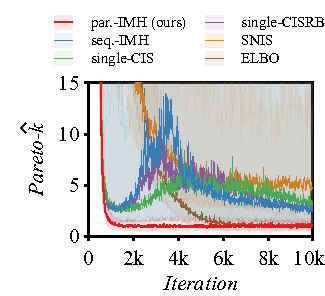
\includegraphics[scale=0.80]{figures/pima_01.pdf}
  }
  \subfloat[Heart]{
    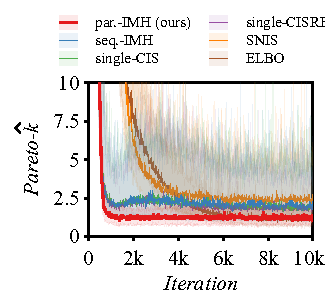
\includegraphics[scale=0.80]{figures/heart_01.pdf}
  }
  \caption{Pareto-\(\widehat{k}\) results of logistic regression problems.
    The solid lines are the median of 100 repetitions while the colored regions are the 80\% empirical percentiles.
  }
\end{figure}

%%% Local Variables:
%%% TeX-master: "master"
%%% End:


\section{Pseudocodes}
\subsection{Markov Chain Kernels}


  \begin{center}
\begin{minipage}[c]{0.63\textwidth}
  \begin{algorithm2e}[H]
    \DontPrintSemicolon
    \SetAlgoLined
    \KwIn{previous sample \(\vz_{t-1}\),
      previous parameter \(\vlambda_{t-1}\),
      number of proposals \(N\)
    }
    \(\vz^{(0)} = \vz_{t-1}\) \;
    \(\vz^{(i)} \sim q_{\text{def.}}\left(\vz;\vlambda_{t-1}\right)\quad\) for \(i = 1, 2,\ldots, N\) \;
    \(\widetilde{w}(\vz^{(i)}) = p(\vz^{(i)},\vx) \,/\, q_{\text{def.}}\left(\vz^{(i)}; \vlambda_{t-1}\right)\quad\) for \(i = 0, 1,\ldots, N\)\;
    \(\overline{w}^{(i)} = \nicefrac{\widetilde{w}(\vz^{(i)})}{ \sum^{N}_{i=0} \widetilde{w}(\vz^{(i)}) }\quad\) for \(i = 0, 1,\ldots, N\)\;
    \(\vz_{t} \sim \mathrm{Multinomial}(\overline{w}^{(0)}, \overline{w}^{(1)}, \ldots, \overline{w}^{(N)}) \)\;
    \caption{Conditional Importance Sampling Kernel}
  \end{algorithm2e}
\end{minipage}
  \end{center}

  \begin{center}
\begin{minipage}[c]{0.62\textwidth}
  \begin{algorithm2e}[H]
    \DontPrintSemicolon
    \SetAlgoLined
    \KwIn{previous sample \(\vz_{t-1}\),
      previous parameter \(\vlambda_{t-1}\),
    }
    \(\vz^* \sim q_{\text{def.}}\left(\vz; \vlambda_{t-1}\right)\)\;
    \(w(\vz) = p(\vz,\vx)/q_{\text{def.}}\left(\vz; \vlambda_{t-1}\right) \)\;
    \(\alpha = \min\left( w\,(\vz^*)/w\,(\vz_{t-1}), 1\right)\)\;
    \(u \sim \mathrm{Uniform}(0, 1) \)\;
    \eIf{u < \(\alpha\)}
        {
          %\(\vz_t \leftarrow \vz^*\)
          \(\vz_t = \vz^*\)
        }
        {
          %\(\vz_t \leftarrow \vz_{t-1}\)
          \(\vz_t = \vz_{t-1}\)
        }
        \caption{Independent Metropolis-Hastings Kernel}
  \end{algorithm2e}
\end{minipage}
  \end{center}

\subsection{Markov Chain Score Ascent Algorithms}

\begin{center}
\begin{minipage}[c]{0.6\textwidth}
  \centering
  \begin{algorithm2e}[H]
    \DontPrintSemicolon
    \SetAlgoLined
    \KwIn{MCMC kernel \(K_{\vlambda}(\vz,\cdot)\),
      initial sample \(\vz_0\),
      initial parameter \(\vlambda_0\),
      number of iterations \(T\),
      stepsize schedule \(\gamma_t\)}
    \For{\textcolor{black}{\(t = 1, 2, \ldots, T\)}}{
      \( \vz_{t} \sim K_{\vlambda_{t-1}}(\vz_{t-1}, \cdot) \)\;
      \(\vs\,(\vlambda; \vz) = \nabla_{\vlambda} \log q\,(\vz; \vlambda)\)\;
      \( \vg_{\text{single}} = s\,(\vlambda_{t-1}; \vz_{t}) \)\;
      \( \vlambda_{t} = \vlambda_{t-1} + \gamma_t\, \vg_{\text{single}} \)\;
    }
    \caption{Markovian Score Climbing}\label{alg:msc}
  \end{algorithm2e}
\end{minipage}
\end{center}

  \begin{center}
  \begin{minipage}[c]{0.63\textwidth}
    \begin{algorithm2e}[H]
      \DontPrintSemicolon
      \SetAlgoLined
      \KwIn{MCMC kernel \(K_{\vlambda}(\vz,\cdot)\),
        initial sample \(\vz_0^{(N)}\),
        initial parameter \(\vlambda_0\),
        number of iterations \(T\),
        stepsize schedule \(\gamma_t\)
      }
      \For{\(t = 1, 2, \ldots, T\)}{
        \(\vz_{t}^{(0)} = \vz_{t-1}^{(N)}\)\;
        \For{\(n = 1, 2, \ldots, N\)}{
          \(\vz_{t}^{(n)} \sim K_{\vlambda_{t-1}}(\vz_{t}^{(n-1)}, \cdot)\)\;
        }
        \( \vs\left(\vlambda; \vz\right) = \nabla_{\vlambda} \log q\,(\vz; \vlambda) \)\;
        \( \vg = \frac{1}{N} \sum^{N}_{n=1} \vs\,(\vlambda_{t-1}; \vz_{t}^{(n)}) \)\;
        \( \vlambda_{t} = \vlambda_{t-1} + \gamma_t \, \vg \,
        \)\;
      }
      \caption{Joint Stochastic Approximation}\label{alg:jsa}
    \end{algorithm2e}
  \end{minipage}
  \end{center}

  \begin{center}
\begin{minipage}[c]{0.7\textwidth}
  \begin{algorithm2e}[H]
    \DontPrintSemicolon
    \SetAlgoLined
    \KwIn{MCMC kernel \(K_{\vlambda}(\vz,\cdot)\),
      initial samples \(\vz_0^{(1)},\, \ldots,\, \vz_0^{(N)}\),
      initial parameter \(\vlambda_0\),
      number of iterations \(T\),
      stepsize schedule \(\gamma_t\)
    }
    \For{\(t = 1, 2, \ldots, T\)}{
        \For{\(n = 1, 2, \ldots, N\)}{
          \(\vz^{(n)}_{t} \sim K_{\vlambda_{t-1}}(\vz^{(n)}_{t-1}, \cdot)\)\;
      }
      \( \vs\left(\vlambda; \vz\right) = \nabla_{\vlambda} \log q\,(\vz;\vlambda) \)\;
      \( \vg = \frac{1}{N} \sum^{N}_{i=1} \vs\,(\vlambda_{t-1}; \vz_{t}^{(i)}) \)\;
      \( \vlambda_{t} = \vlambda_{t-1} + \gamma_t\, \vg \)\;
    }
    \caption{Parallel Markov Chain Score Ascent}\label{alg:pmcsa}
  \end{algorithm2e}
\end{minipage}
  \end{center}

%%% Local Variables:
%%% TeX-master: "master"
%%% End:


\subsection{Isotropic Gaussian Experiments}
\begin{figure}[H]
  \centering
  \subfloat[\(N=2^2\)]{
    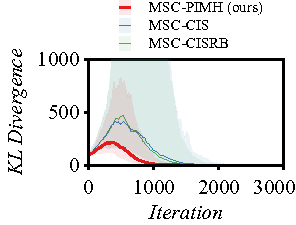
\includegraphics[scale=0.75]{figures/gaussian_01.pdf}
  }
  \subfloat[\(N=2^4\)]{
    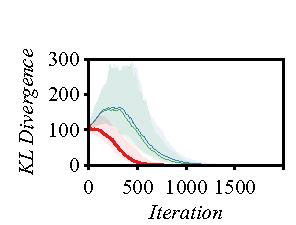
\includegraphics[scale=0.75]{figures/gaussian_02.pdf}
  }
  \subfloat[\(N=2^6\)]{
    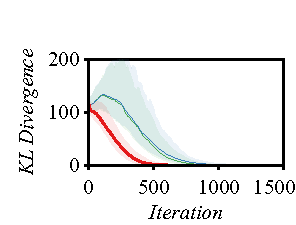
\includegraphics[scale=0.75]{figures/gaussian_03.pdf}
  }
  \caption{100-D isotropic Gaussian example with a varying computational budget \(N\).
    MSC-PIMH converges faster than MSC-CIS and MSC-CISRB regardless of \(N\).
    Also, the convergence of MSC-PIMH becomes more stable/monotonic as \(N\) increases.
    The solid lines and colored regions are the medians and 80\% percentiles computed from 100 repetitions.
  }\label{fig:gaussian}
\end{figure}
%
We perform experiments with an 100-D isotropic multivariate Gaussian distribution.
With Gaussian distributions, convergence can be evaluated exactly since their KL divergence is available in a closed form.
We compare the performance of MSC-PIMH, MSC-CIS, and MSC-CISRB with respect to the \(N\) (number of proposals for MSC-CIS, MSC-CISRB; number of parallel chains for MSC-PIMH).
The results are shown in~\cref{fig:gaussian}.
While MSC-PIMH shows some level of overshoot wih \(N=4\), it shows monotonic convergence with larger \(N\).
On the other hand, both MSC-CIS and MSC-CISRB overshoots even with \(N=64\).
This clearly shows that our PIMH kernel enjoys better gradient estimates compared to the CIS kernel.

\subsection{Numerical Simulation}
We now present numerical simulations of our analyses in~\cref{section:bias_variance} and~\cref{section:cis_bias}.
In particular, we visualize the fact that the variance of the CIS kernel can increase with the number of proposals \(N\) when the KL divergence is large, as described in~\eqref{eq:cis_variance_incr}.

\paragraph{Experimental Setup}
We first set the target distribution as \(p\,(z \mid x) = \mathcal{N}(0, 1)\) and the proposal distribution as \(q\,(z; \mu) = \mathcal{N}(\mu, 2)\) with varying mean.
We measure the variance of estimating the score function \(s\,(z, \mu) = \frac{\partial q(\vz; \mu)}{\partial \mu} \) using the CIS, CISRB, and PIMH kernels, given the previous Markov-chain state \(z_{t-1}\) and computational budget \(N\).
For CIS and CISRB, we set a fixed \(z_{t-1}\), while for PIMH, we randomly sample \(N\) samples from \(\vz_{t-1} \sim p\,(z \mid z)\) (we obtained similar trends regardless of the distribution of \(z_{t-1}\)).
The variance is estimated using \(2^{14}\) samples from \(K(\vz_{t-1}, \cdot)\).
We report the variance across varying \(N\) and varying KL divergence between \(q_{\vlambda}(z)\) and \(p\,(\vz\mid\vx)\).
The latter is performed by varying the difference between the mean of the proposal and the target distributions \(\Delta \mu = \Esub{p(\vz\mid\vx)}{z} - \Esub{q_{\vlambda}}{z} \).

\begin{figure}[H]
  \centering
  \subfloat[\(\Delta \mu = 0\)]{
    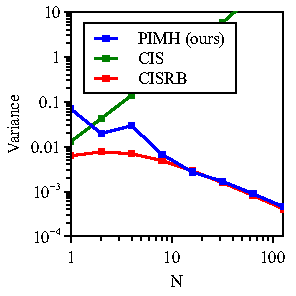
\includegraphics[scale=0.85]{figures/simulations_01.pdf}
  }
  \subfloat[\(\Delta \mu = 2\)]{
    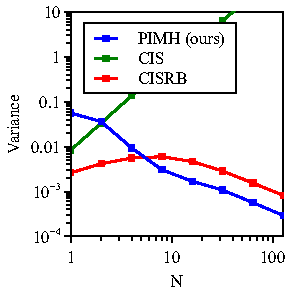
\includegraphics[scale=0.85]{figures/simulations_02.pdf}
  }
  \subfloat[\(\Delta \mu = 4\)]{
    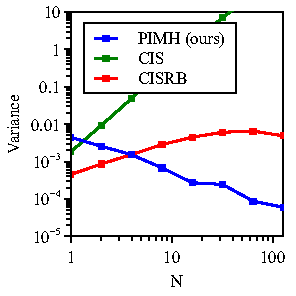
\includegraphics[scale=0.85]{figures/simulations_03.pdf}
  }
  \caption{Conditional variance of different MCMC kernels with varying \(N\) and varying difference between the mean of the target and proposal distributions.
  }\label{fig:simulations}
  \vspace{-0.1in}
\end{figure}

\paragraph{Results Summary}
The results are presented in Figure~\ref{fig:simulations}.
We can see that, when the difference of the mean of the \(p\) and \(q\) is large, the variance of CISRB \textit{increases} with \(N\).
This increasing trend becomes stronger as the KL divergence between \(p\) and \(q\) increases.
While this simulation suggests that CISRB has much smaller variance compared to CIS, our realistic experiments in~\cref{section:eval} did not reveal such levels of performance gains.
Is also visible that PIMH has a slightly larger variance compared to \(CIS\) in the small \(N\) regime.
This is due to the higher acceptance rate of the Metropolis-Hastings acceptance ratio compared to Barker's acceptance ratio used by CIS~\citep{peskun_optimum_1973, minh_understanding_2015}.

%%% Local Variables:
%%% TeX-master: "master"
%%% End:


\subsection{Probabilistic Models Used in Experiments}
We present the probabilistic models used in our experiments in~\cref{section:eval}.

\subsubsection{Hierarchical Logistic Regression}
\begin{align*}
    \sigma_{\beta}  &\sim \mathcal{N}^+\left(0, 1.0\right) \\
    \sigma_{\alpha} &\sim \mathcal{N}^+\left(0, 1.0\right) \\
    \symbf{\beta} &\sim \mathcal{N}\left(\symbf{0}, \sigma_{\beta}^2\,\symbf{I}\right) \\
    \alpha        &\sim \mathcal{N}\left(0, \sigma_{\alpha}^2\right) \\
    p             &\sim \mathcal{N}\left(\vx_i^{\top}\symbf{\beta} + \alpha,\, \sigma_{\alpha}^2\right)\\
    y_i           &\sim \text{Bernoulli-Logit}\,(p)
\end{align*}

\subsubsection{Stochastic Volatility}
\begin{align*}
    \mu    &\sim \mathrm{Cauchy}(0, 10) \\
    \phi   &\sim \mathrm{Uniform}\,(-1, 1) \\
    \sigma &\sim \mathrm{Cauchy}^+(0, 5) \\
    h_1    &\sim \mathcal{N}\left( 0, \frac{\sigma^2}{1 - \phi^2} \right) \\
    h_{t+1} &\sim \mathcal{N}\left( \mu + \phi\,\left( h_{t} - \mu \right), \sigma^2 \right) \\
    y_t    &\sim \mathcal{N}\left( 0, \exp\left( h_{t} \right) \right)
\end{align*}
\(y_t\) is the stock price at the \(t\)th point in time.

\subsubsection{Radon Hierarchical Regression}
\begin{align*}
  \sigma_{a_1} &\sim \mathrm{Gamma}\left( \alpha = 1, \beta = 0.02 \right) \\
  \sigma_{a_2} &\sim \mathrm{Gamma}\left( \alpha = 1, \beta = 0.02 \right) \\
  \sigma_{y}  &\sim \mathrm{Gamma}\left( \alpha = 1, \beta = 0.02 \right) \\
  \mu_{a_1}    &\sim \mathcal{N}\left( 0, 1 \right) \\
  \mu_{a_2}    &\sim \mathcal{N}\left( 0, 1 \right) \\
  a_{1,\, c}     &\sim \mathcal{N}\left( \mu_{a_1}, \sigma_{a_1}^2 \right) \\
  a_{2,\, c}     &\sim \mathcal{N}\left( \mu_{a_2}, \sigma_{a_2}^2 \right) \\
  y_i         &\sim \mathcal{N}\left( a_{1,\, c_i} + a_{2,\, c_i}\,x_i,\, \sigma_y^2 \right)
\end{align*}
\(a_{1,\,c}\) is the intercept at the county \(c\), \(a_{2,\,c}\) is the slope at the county \(c\), \(c_i\) is the county of the \(i\)th datapoint, \(x_i\) is the floor predictor of the measurement, and \(y_i\) is the measured radon level.

%% \begin{align}
%% Turing.@model radon(county, x, y) = begin
%%     σ_a1 ~ Gamma(1, 50)
%%     σ_a2 ~ Gamma(1, 50)
%%     σ_y  ~ Gamma(1, 50)
%%     μ_a1 ~ Normal(0,1)
%%     μ_a2 ~ Normal(0,1)

%%     a1   ~ MvNormal(fill(μ_a1, 85), fill(σ_a1, 85))
%%     a2   ~ MvNormal(fill(μ_a2, 85), fill(σ_a2, 85))

%%     μ_y  = a1[county] + a2[county].*x
%%     y    ~ MvNormal(μ_y, σ_y)
%% end
%% \end{align}

%%% Local Variables:
%%% TeX-master: "master"
%%% End:


%\newpage
\section{Proofs}
%

\textit{Detailed derivation of \textbf{\cref{eq:cis_kernel}}}
\begin{proof}[\unskip\nopunct]
\begin{align}
  &\Esub{K(\vz_{t-1}, \vz)}{f(\vz)} \\
  &= \Esub{q_{\vlambda}}{
      \sum^{N}_{i=0} w\,(\vz^{(i)}) f(\vz^{(i)}) 
      \,/\,
      \sum^{N}_{i=0} w\,(\vz^{(i)})
  } \\
  \intertext{
    (with a slight abuse of notation, \(\vz_{t-1} = \vz^{(0)}\))
  }
  &= \Esub{q_{\vlambda}}{
    \Big(
    \sum^{N}_{i=1} w\,(\vz^{(i)})\,f(\vz^{(i)}) + w\,(\vz_{t-1}) f(\vz_{t-1})
    \Big)
      \,/\,
      \sum^{N}_{i=0} w\,(\vz^{(i)})
  } \\
  &= \Esub{q_{\vlambda}}{
    \frac{
      \sum^{N}_{i=1} w\,(\vz^{(i)})\,f(\vz^{(i)})
    }
    {
      \sum^{N}_{i=0} w\,(\vz^{(i)})
    }
    +
    \frac{w\,(\vz_{t-1})}{\sum^{N}_{i=0} w\,(\vz^{(i)})} f(\vz_{t-1})
  } \\
  &= \Esub{q_{\vlambda}}{
    \frac{
      \sum^{N}_{i=1} w\,(\vz^{(i)})  
    }
    {
      \sum^{N}_{i=0} w\,(\vz^{(i)})  
    }
    \frac{
      \sum^{N}_{i=1} w\,(\vz^{(i)})\,f(\vz^{(i)})
    }
    {
      \sum^{N}_{i=1} w\,(\vz^{(i)})
    }
    +
    \frac{w\,(\vz_{t-1})}{\sum^{N}_{i=0} w\,(\vz^{(i)})} f(\vz_{t-1})
  } \\
  &= \Esub{q_{\vlambda}}{
    \left(
    1 - \frac{
       w\,(\vz_{t-1}) 
    }
    {
      \sum^{N}_{i=0} w\,(\vz^{(i)})  
    }
    \right)\,
    \frac{
      \sum^{N}_{i=1} w\,(\vz^{(i)})\,f(\vz^{(i)})
    }
    {
      \sum^{N}_{i=1} w\,(\vz^{(i)})
    }
    +
    \frac{w\,(\vz_{t-1})}{\sum^{N}_{i=0} w\,(\vz^{(i)})} f(\vz_{t-1})
  } \\
  &= \Esub{q_{\vlambda}}{
    \alpha\,(\vz_{t-1}, \vz^{(1:N)}) \,
    \frac{
      \sum^{N}_{i=1} w\,(\vz^{(i)})\,f(\vz^{(i)})
    }
    {
      \sum^{N}_{i=1} w\,(\vz^{(i)})
    }
    +
    r\,(\vz_{t-1}\mid\vz^{(1:N)}) \, f(\vz_{t-1})
  }\label{eq:cis_kernel_inter} \\ 
  \intertext{where we denote
    \(
    \alpha\,(\vz_{t-1}, \vz^{(1:N)}) =
    \frac{
      \sum^{N}_{i=1} w\,(\vz^{(i)})  
    }
    {
      \sum^{N}_{i=0} w\,(\vz^{(i)})  
    }
  \),
  \(
  r\,(\vz_{t-1}\mid\vz^{(1:N)}) = \frac{w\,(\vz_{t-1})}{\sum^{N}_{i=0} w\,(\vz^{(i)})}
  \), and thus,
  }
%
  &= \Esub{q_{\vlambda}}{
    \alpha\,(\vz_{t-1}, \vz^{(1:N)}) \,
    \frac{
      \sum^{N}_{i=1} w\,(\vz^{(i)})\,f(\vz^{(i)})
    }
    {
      \sum^{N}_{i=1} w\,(\vz^{(i)})
    }
  }
    +
 \Esub{q_{\vlambda}}{
   r\,(\vz_{t-1}\mid\vz^{(1:N)})
 } f(\vz_{t-1}) \\
%
  &= \Esub{q_{\vlambda}}{
    \alpha\,(\vz_{t-1}, \vz^{(1:N)}) \,
    \frac{
      \sum^{N}_{i=1} w\,(\vz^{(i)})\,f(\vz^{(i)})
    }
    {
      \sum^{N}_{i=1} w\,(\vz^{(i)})
    }
  }
    +
   r\,(\vz_{t-1})\,f(\vz_{t-1}) %\\
%
  %% &=  
  %%  \int \alpha\,(\vz_{t-1}, \vz^{(1:N)}) \,
  %%   \frac{
  %%     \sum^{N}_{i=1} w\,(\vz^{(i)})\,f(\vz^{(i)})
  %%   }
  %%   {
  %%     \sum^{N}_{i=1} w\,(\vz^{(i)})
  %%   } \,
  %%   q_{\vlambda}(\vz^{(1:N)})\,d\vz^{(1:N)}
  %%   +
  %%  r\,(\vz_{t-1})\,f(\vz_{t-1})
\end{align}
\end{proof}

%%% Local Variables:
%%% TeX-master: "master"
%%% End:

\printProofs

\end{document}
